\documentclass[13pt,a4paper,font=cm]{report}
% \usepackage{vntex}
\usepackage[vietnamese]{babel}
\usepackage[caption=false, font=footnotesize]{subfig}
\usepackage{times}

\usepackage{notoccite}


%\usepackage[english,vietnam]{babel}
%\usepackage[utf8]{inputenc}
\usepackage{mathptmx}[ptm]
\usepackage{indentfirst}
%\usepackage[utf8]{inputenc}
%\usepackage[francais]{babel}
\usepackage{a4wide,amssymb,epsfig,latexsym,array,hhline,fancyhdr}

\usepackage[normalem]{ulem}
%\usepackage{soul}
\usepackage{setspace}
\usepackage{longtable}

\usepackage{algpseudocode}

\usepackage[makeroom]{cancel}
\usepackage{amsmath}
\usepackage{amsthm}
\usepackage{multicol,longtable,amscd}
\usepackage{diagbox}%Make diagonal lines in tables
\usepackage{booktabs}
\usepackage{alltt}
\usepackage[framemethod=tikz]{mdframed}% For highlighting paragraph backgrounds
\usepackage[font={12pt},margin=1cm]{caption,subcaption}
% \usepackage[font={12pt},margin=1cm]{caption}
\usepackage{lastpage}
\usepackage{algorithm}
\usepackage{enumerate}
\usepackage{color}
\usepackage{graphicx}							% Standard graphics package
\usepackage{array}
\usepackage{tabularx, caption}
\usepackage{multirow}
\usepackage{multicol}
\usepackage{rotating}
\usepackage{graphics}
\usepackage{geometry}
\usepackage{setspace}
\usepackage{epsfig}
\usepackage{tikz}
\renewcommand{\thesubsubsection}{\thesubsection.\alph{subsubsection}}

\usetikzlibrary{arrows,snakes,backgrounds,calc}
\usepackage[unicode]{hyperref}
\hypersetup{urlcolor=blue,linkcolor=black,citecolor=black,colorlinks=true} 
\usepackage{listings}

%\usepackage{pstcol} 				
% PSTricks with the standard color package

\usepackage[normalem]{ulem}

\usepackage{titlesec}
\usepackage[nocompress]{cite}
\usepackage{times}
% \bibliographystyle{unsrt}
% %AUTHOR%%
\author{Hoang Khang PHAN}


\counterwithin{figure}{chapter}
\counterwithin{table}{chapter}
\counterwithin{algorithm}{chapter}
\titleformat{\section}  % which section command to format
  {\fontsize{13}{16}\bfseries} % format for whole line
  {\thesection} % how to show number
  {1em} % space between number and text
  {} % formatting for just the text
  [] % formatting for after the text

\titleformat{\subsection}  % which section command to format
  {\fontsize{13}{16}\bfseries} % format for whole line
  {\thesubsection} % how to show number
  {2em} % space between number and text
  {}% formatting for just the text
  [] % formatting for after the text
\titleformat{\subsubsection}  % which section command to format
{\fontsize{13}{16}\bfseries} % format for whole line
{\thesubsubsection} % how to show number
{2em} % space between number and text
{}% formatting for just the text
[] % formatting for after the text

\titleformat{\paragraph}  % which section command to format
{\fontsize{13}{16}\bfseries} % format for whole line
{\theparagraph} % how to show number
{2em} % space between number and text
{}% formatting for just the text
[] % formatting for after the text



\newtheorem{theorem}{{\bf Định lý}}
\newtheorem{property}{{\bf Tính chất}}
\newtheorem{proposition}{{\bf Mệnh đề}}
\newtheorem{corollary}[proposition]{{\bf Hệ quả}}
\newtheorem{lemma}[proposition]{{\bf Bổ đề}}
\theoremstyle{definition}
\newtheorem{exer}{Bài toán}
\addtocontents{toc}{\protect\thispagestyle{empty}}
% Remove page number in contents page. 

\addtocontents{lof}{\protect\thispagestyle{empty}}
% Remove page number in list of figure page. 
\addtocontents{lot}{\protect\thispagestyle{empty}}
% Remove page number in list of table page. 
\def\thesislayout{	% A4: 210 × 297
	\geometry{
		a4paper,
		total={160mm,240mm},  % fix over page
		left=30mm,
		top=22mm,
            right=20mm,
            bottom=20mm,
	}
}
\def\thesisheadlayout{	% A4: 210 × 297
	\geometry{
		a4paper,
		total={160mm,240mm},  % fix over page
		left=30mm,
		top=10mm,
	}
}

\thesislayout
\lstset{
language=R,
basicstyle=\footnotesize\sffamily,
commentstyle=\ttfamily\color{black},
numbers=left,
numberstyle=\ttfamily\color{black}\footnotesize,
stepnumber=1,
numbersep=5pt,
backgroundcolor=\color{white},
showspaces=false,
showstringspaces=false,
showtabs=false,
frame=single,
tabsize=2,
captionpos=b,
breaklines=true,
breakatwhitespace=false,
title=\lstname,
escapeinside={},
keywordstyle={},
morekeywords={}
}
\usepackage{fancyhdr}
\setlength{\headheight}{40pt}
\pagestyle{fancy}
 % clear all header fields
\renewcommand{\footruleskip}{1mm}

\fancyhead[L]{
 \begin{tabular}{rl}
   %  \begin{picture}(25,15)(0,0)
   %  \put(0,-8){
\includegraphics[width=10mm, height=10mm]{Images/hcmut.png}}
   %  %\put(0,-8){\epsfig{width=10mm,figure=hcmut.eps}}
   % \end{picture}&
	%
\includegraphics[width=8mm, height=8mm]{hcmut.png} & %
	\begin{tabular}{l}
		\textbf{  Trường Đại Học Bách Khoa - Đại học Quốc gia TP.HCM }\\
		\textbf{  Khoa Khoa Học Ứng Dụng}
	\end{tabular} 	
 \end{tabular}
}
\fancyhead[R]{ \textbf{Báo cáo Đồ án chuyên ngành} } % clear all footer fields
\fancyfoot[L]{\scriptsize  SVTH: Phan Hoàng Khang}
\fancyfoot[R]{\scriptsize GVHD: Ths Lê Nhật Tân\\  Trang {\thepage}/\pageref{LastPage}}

\renewcommand{\headrulewidth}{0.3pt}
\renewcommand{\footrulewidth}{0.3pt}

%%%
\setcounter{secnumdepth}{4}
\setcounter{tocdepth}{3}
\makeatletter
\newcounter {subsubsubsection}[subsubsection]
\renewcommand\thesubsubsubsection{\thesubsubsection .\@alph\c@subsubsubsection}
\newcommand\subsubsubsection{\@startsection{subsubsubsection}{4}{\z@}%
                                     {-3.25ex\@plus -1ex \@minus -.2ex}%
                                     {1.5ex \@plus .2ex}%
                                     {\normalfont\normalsize\bfseries}}
\newcommand*\l@subsubsubsection{\@dottedtocline{3}{10.0em}{4.1em}}
\newcommand*{\subsubsubsectionmark}[1]{}
\makeatother

\everymath{\color{black}}%make in-line maths symbols blue to read/check easily

\sloppy
\captionsetup[figure]{labelfont={Large,bf},textfont={Large,it},belowskip=-1pt}
%space remove between caption, figure, and text
\captionsetup[table]{labelfont={Large,bf},textfont={Large,it},belowskip=-1pt}
\captionsetup[algorithm]{labelfont={Large,bf},textfont={Large,it},belowskip=-1pt}
\setlength{\floatsep}{5pt plus 2pt minus 2pt}
\setlength{\textfloatsep}{5pt plus 2pt minus 2pt}
\setlength{\intextsep}{10pt plus 2pt minus 2pt}

\thesislayout

\begin{document}

\begin{titlepage}
\begin{tikzpicture}[remember picture, overlay]
  \draw[line width = 4pt] ($(current page.north west) + (0.4in,-0.5in)$) rectangle ($(current page.south east) + (-0.4in,0.5in)$);
  \draw[line width=1.5pt]
    ($ (current page.north west) + (0.45in,-0.55in) $)
    rectangle
    ($ (current page.south east) + (-0.45in,0.55in) $);
\end{tikzpicture}

\begin{center}
\LARGE \textbf{ĐẠI HỌC QUỐC GIA THÀNH PHỐ HỒ CHÍ MINH} \\
\vspace{0.2cm}
\LARGE \textbf{TRƯỜNG ĐẠI HỌC BÁCH KHOA} \\
\vspace{0.2cm}
\LARGE \textbf{KHOA KHOA HỌC ỨNG DỤNG}
\end{center}

\vspace{0.3cm}

\begin{figure}[h!]
\begin{center}

\includegraphics[width=6cm]{Images/hcmut.png}
\end{center}
\end{figure}

\begin{center}
\begin{tabular}{c}
\multicolumn{1}{c}{\textbf{{\LARGE ĐỒ ÁN CHUYÊN NGÀNH}}}\\
\\{\textbf{{\Huge }}}
% \\{\textbf{{\LARGE ĐỒ ÁN KỸ THUẬT MÁY TÍNH}}}
% \\{\textbf{{\LARGE ĐỒ ÁN MÔN HỌC}}}
% \\ \textit{(SV chọn tên môn học cho phù hợp)}
\\
\\
% \textbf{\Huge TÊN ĐỀ TÀI}
\\ \textbf{\Huge Phân tích hành vi di chuyển của sinh viên } \\ \textbf{\Huge giành cho nhận diện stress hằng ngày}
\\
\\
\\
\\
\\
\\
\\
\\

\\ \vspace{0.5cm} {\textbf{{\LARGE Phan Hoàng Khang}}}
\end{tabular}
\end{center}
% \vspace{0.5cm}
% \begin{table}[h]
% \begin{tabular}{rll}
% \hspace{6 cm} &  \textbf{\Large HỘI ĐỒNG:} {\Large ................................}
% \\
% \\
% \hspace{6 cm} &   \textbf{\Large GVHD:} {\Large Lê Nhật Tân}
% \\
% \\
% \hspace{6 cm}  &   \textbf{\Large TKHĐ:} {\Large ................................}
% \\
% \\
% % TKHĐ là THƯ KÝ HỘI ĐỒNG
% \hspace{6 cm} &     \textbf{$\;$ $\;$$\;$$\;$$\;$$\;$$\;$$\;$$\;$$\;$$\;$$\;$$\;$$\;$$\;$$\;$$\;$$\;$$\;$$\;$$\;$$\;$$\;$$\;$$\;$$\;$$\;$$\;$$\;$$\;$$\;$$\;$$\;$$\;$ \Large ---o0o---} 
% \\
% \\
% \hspace{6 cm} &   \textbf{\Large SVTH1:} {\Large Phan Hoàng Khang (2111460)}
% \\
% \\
% \hspace{6 cm}&   \textbf{\Large SVTH2:}  {\Large .....Họ \& Tên...........(MSSV)}
% \\
% \\
% \hspace{6 cm} &   \textbf{\Large SVTH3:}  {\Large .....Họ \& Tên...........(MSSV)}
% \\
% \\
% \end{tabular}
% \end{table}
\vspace{0.5cm}
\begin{center}
{\Large TP. HỒ CHÍ MINH, 12/2024 }
\end{center}
\end{titlepage}
\thispagestyle{empty}
\newpage


%%%%%%%%2nd PAGE%%%%%%%%%%%%%%%%%%%
\begin{titlepage}


\begin{center}
\LARGE \textbf{ĐẠI HỌC QUỐC GIA THÀNH PHỐ HỒ CHÍ MINH} \\
\vspace{0.2cm}
\LARGE \textbf{TRƯỜNG ĐẠI HỌC BÁCH KHOA} \\
\vspace{0.2cm}
\LARGE \textbf{KHOA KHOA HỌC ỨNG DỤNG}
\end{center}

\vspace{0.3cm}

\begin{figure}[h!]
\begin{center}

\includegraphics[width=6cm]{Images/hcmut.png}
\end{center}
\end{figure}

\begin{center}
\begin{tabular}{c}
\multicolumn{1}{c}{\textbf{{\LARGE ĐỒ ÁN CHUYÊN NGÀNH}}}\\
\\{\textbf{{\Huge }}}
% \\{\textbf{{\LARGE ĐỒ ÁN KỸ THUẬT MÁY TÍNH}}}
% \\{\textbf{{\LARGE ĐỒ ÁN MÔN HỌC}}}
% \\ \textit{(SV chọn tên môn học cho phù hợp)}
\\
\\
% \textbf{\Huge TÊN ĐỀ TÀI}
\\ \textbf{\Huge Phân tích hành vi di chuyển của sinh viên } \\ \textbf{\Huge giành cho nhận diện stress hằng ngày}
\\
\\
\\
\\


\\ \vspace{0.5cm} {\textbf{{\LARGE Ngành: Vật Lý Kỹ Thuật (7520401)}}}
\end{tabular}
\end{center}
% \vspace{0.5cm}
\begin{table}[h]
\begin{tabular}{rll}
\hspace{6 cm} &  \textbf{\Large Sinh Viên:} {\Large Phan Hoàng Khang}
\\
\\
\hspace{6 cm} &   \textbf{\Large MSSV:} {\Large 2111460 }
\\
\\
\hspace{6 cm}  & \textbf{\Large GVHD:} {\Large Lê Nhật Tân }\\
\hspace{8 cm}  & {$\;\;\;\;\;\;\;\;\;\;\;\;\;\;\;\;\;\;\;\;\;\;$ \Large GVHD2 } % don't remove $\;$
\\
\\
% TKHĐ là THƯ KÝ HỘI ĐỒNG
% \hspace{6 cm} &     \textbf{$\;$ $\;$$\;$$\;$$\;$$\;$$\;$$\;$$\;$$\;$$\;$$\;$$\;$$\;$$\;$$\;$$\;$$\;$$\;$$\;$$\;$$\;$$\;$$\;$$\;$$\;$$\;$$\;$$\;$$\;$$\;$$\;$$\;$$\;$ \Large ---o0o---} 
\\
\\
% \hspace{6 cm} &   \textbf{\Large SVTH1:} {\Large Phan Hoàng Khang (2111460)}
% \\
% \\
% \hspace{6 cm}&   \textbf{\Large SVTH2:}  {\Large .....Họ \& Tên...........(MSSV)}
% \\
% \\
% \hspace{6 cm} &   \textbf{\Large SVTH3:}  {\Large .....Họ \& Tên...........(MSSV)}
\\
\\
\end{tabular}
\end{table}
\vspace{0.5cm}
\begin{center}
{\Large TP. HỒ CHÍ MINH, 12/2024 }
\end{center}
\end{titlepage}
\thispagestyle{empty}
\floatname{algorithm}{Mã giả}
\renewcommand{\listalgorithmname}{Danh sách mã giả}
\newpage
%%%%%%%%%%%%%%%%%INTRO%%%%%%%%%%%%%%%%%%%

\linespread{1.25}
% \section*{Lời cảm ơn}
\thispagestyle{empty}

I like to acknowledge ...

\clearpage
\pagenumbering{arabic}

% \section*{Lời cam đoan}
\thispagestyle{empty}

I like to acknowledge ...

\clearpage
\pagenumbering{arabic}

\section*{Tóm tắt}
\thispagestyle{empty}
\fontsize{13}{16}
\selectfont
Căng thẳng tâm lý, một rối loạn tâm lý phổ biến, có ảnh hưởng tiêu cực đáng kể đến chất lượng cuộc sống và hiệu suất công việc, đặc biệt đối với sinh viên đang chịu áp lực phải học tập tốt. Quản lý tốt vấn đề tâm lý này là điều cần thiết để giảm thiểu hậu quả tiêu cực và cho phép can thiệp kịp thời. Nghiên cứu này sử dụng dữ liệu điện thoại thông minh - một công cụ phổ biến trong cuộc sống hiện đại - để phát triển một phương pháp mạnh mẽ để giám sát và quản lý căng thẳng từ xa.

Trong nghiên cứu này, các đặc điểm thống kê dựa trên thời lượng cuộc trò chuyện và thời lượng tĩnh; vị trí liên quan đến các số liệu dựa trên thời gian (thời gian ở trường, ở nhà, đi ăn ngoài, v.v. vào buổi sáng, trưa hoặc cả ngày) thu được từ dữ liệu GPS; tình trạng di chuyển liên quan đến các tính năng thời gian (thời gian di chuyển, thời gian hoạt động giải trí, v.v. vào buổi sáng, trưa hoặc cả ngày); ước tính các trường hợp bỏ lớp bằng cách căn chỉnh lịch học với vị trí của sinh viên; thời hạn sắp tới của sinh viên; và các tính năng dựa trên thời gian như cosin của ngày trong tuần và tuần số trong học kỳ được trích xuất từ bộ dữ liệu StudentLife.

Việc phát hiện căng thẳng đã được thử nghiệm trong hai trường hợp phân loại hai lớp (căng thẳng/không căng thẳng) và phân loại ba lớp (cảm thấy hạnh phúc, căng thẳng một chút và căng thẳng). Trong cả hai trường hợp, chúng tôi đã thử nghiệm ba mô hình học máy phổ biến: SVM, XGBoost và Random Forest. Kết quả cho thấy, trong phân loại hai lớp, hiệu suất của Random Forest đạt được độ chính xác lên đến 79\% và điểm F1 macro là 63\% và nó cũng thống trị phân loại ba lớp theo độ chính xác và điểm F1 macro lần lượt là 66\% và 51\%. Hơn nữa, chúng tôi cũng đã sử dụng Shapley Additive exPlanations (SHAP) để đánh giá hiểu biết từ các tính năng được trích xuất này. Kết quả cho thấy tính năng 'tuần trong học kỳ' đặc trưng nhất cho mức độ căng thẳng của sinh viên. Cũng cần lưu ý rằng sinh viên bỏ lớp có khả năng bị căng thẳng cao hơn một chút vào ngày hôm đó và có khả năng bị căng thẳng thấp hơn vào ngày hôm sau so với các sinh viên khác. Những hiểu biết này có giá trị cho nghiên cứu trong tương lai và cung cấp các cách tiếp cận thực tế để phát hiện và quản lý căng thẳng.

\clearpage
\pagenumbering{arabic}

\section*{Abstract}
\thispagestyle{empty}
\fontsize{13}{16}
\selectfont
 Mental stress, a common psychological disorder, has a significantly negative influence on life quality and work performance, especially for students who are under pressure to perform well in school. It is essential to handle this psychological issue well in order to minimize negative consequences and enable timely intervention. This study uses smartphone data - a ubiquitous tool in modern life - to develop a powerful approach to remotely monitor and manage stress. In this research, statistical features based on conversation duration and stationary duration; location with regard to time-based metrics (time spent at school, at home, for dining out, etc. in the morning, noon, or whole day) derived from GPS data; mobility status with respect to time features (moving time, recreational activity time, etc. in the morning, noon, or whole day); estimation of skipped class instances by aligning class schedules with student locations; the upcoming deadlines of student; and time-based features like the cosine of the day of the week and week number in the semester extracted from the StudentLife dataset. The stress detection was tested in two scenarios of two-class classifications (stress/no stress) and three-class classifications (feeling happy, a little stressed, and stressed out). In both scenarios, we tested three popular machine learning models: SVM, XGBoost, and Random Forest. The result shows that, in two-class classifications, the performance of Random Forest reached up to 79\% accuracy and 63\% macro F1 score and it also dominated the three-class classification by the accuracy and macro F1 score of 66\% and 51\% respectively. Moreover, we have also employed Shapley Additive exPlanations (SHAP) to evaluate insights from these extracted features. The results revealed that the 'week in the semester' feature is most characteristic of student stress levels. It is also worth mentioning that students who skip classes have a marginally higher likelihood of experiencing stress on that day, and a lower chance of facing stress the next day compared to their counterparts. These insights are invaluable for future research and offer practical approaches to stress detection and management.

\clearpage
\pagenumbering{arabic}

\newpage
\tableofcontents
\thispagestyle{empty}
\newpage
\listoffigures
\newpage
\listoftables
\newpage
\listofalgorithms
\newpage
\setcounter{page}{1}
%%%%%%%%%%%%%%%%%CONTENTS%%%%%%%%%%%%%%%%%%%
\chapter{Giới thiệu}
\section{Đặt vấn đề}\label{Problems_settings}
Stress tâm lý (hay căng thẳng tâm lý) là một vấn đề phổ biến của thế kỷ 21. Theo nghiên cứu của Cơ quan An toàn và Sức khỏe Nghề nghiệp Anh Quốc, stress chiếm tới 37\% lý do cho các chứng bệnh liên quan đến công việc trong năm 2015/2016
\cite{HSE}. Hơn thế nghiên cứu của Alert cho thấy rằng cứ 3 người Mỹ thì sẽ có 1 người có sức khoẻ tâm thần loại khá hoặc tệ \cite{american_stress}. Về tác hại của căng thẳng, hiện tượng này không chỉ ảnh hưởng đến sức khỏe tinh thần mà còn gây ra nhiều vấn đề về thể chất, như tăng huyết áp, suy giảm hệ miễn dịch, hoặc kiệt quệ. Một nghiên cứu gần đây cho thấy, sinh viên đại học đang đối mặt với mức độ stress cao, dẫn đến giảm hiệu suất học tập và tăng nguy cơ bỏ học. Thêm vào đó theo nghiên cứu của Jeffrey \cite{stress_reduce_productivity}, người bị stress có xu hướng bị giảm 5 đến 12\% năng suất làm việc dẫn đến hơn 50\% giờ làm việc của thế giới đã bị mất hằng năm do các vấn đề tâm lý \cite{workday_lost}. Vì vậy việc nghiên cứu công nghệ để nhận diện stress hằng ngày là quan trọng trong cuộc sống hiện tại.

% Về nghiên cứu về stress tâm lý, một câu hỏi được đặt ra chỉnh là khi nào cần có sự nhận diện vào trạng thái tâm lý của một con người. Để giải quyết vấn đề ấy, ta cần quan tâm đến việc stress là một hiện tượng mà vừa có thể làm động lực cho con người phát triển ở giai đoạn vừa và nhẹ và sẽ gây ra các tác hại khi dần vào các giai đoạn sâu của quá trình ấy. Hơn thế việc can thiệp về tâm lý dặt ra một thách thức về sự thao túng tâm lý của con người.

Khi xét về các ưu điểm việc nhận diện được stress mang lại, các thiết bị đeo được như đồng hồ thông minh đã nổi lên như những công cụ tiềm năng chính xác để phát hiện căng thẳng, tận dụng sự tích hợp của các cảm biến có độ nhạy cao để thu thập các thông số sức khỏe toàn diện. Hơn nữa, với sự phát triển của các công cụ phân tích dữ liệu như học máy và học sâu, dữ liệu sinh trắc trở thành một nguồn thông tin mạnh mẽ để phát hiện căng thẳng chính xác.

Đặc biệt, nhiều nghiên cứu (như nghiên cứu của Pekka Siirtola \cite{PS}, của Salai \cite{stress_heartrate}) đã đạt được độ chính xác ổn trong phát hiện căng thẳng bằng các thiết bị đeo nêu trên. Tuy nhiên, một hạn chế chính nằm ở sự cần thiết phải đeo liên tục, vì dự đoán căng thẳng chính xác bị ảnh hưởng đối với những người chỉ sử dụng thiết bị gián đoạn, chẳng hạn như khi đi lại hoặc tại nơi làm việc.

Điện thoại thông minh, một thiết bị phổ biến trong cuộc sống hiện đại, có tiềm năng đóng vai trò là bộ thu dữ liệu đáng kể để theo dõi căng thẳng liên tục. Ví dụ, Martin Gjoreski và cộng sự đã phát triển một mô hình học máy có thể phát hiện một cách kín đáo mức độ căng thẳng ở sinh viên bằng cách sử dụng dữ liệu có sẵn từ cảm biến điện thoại thông minh\cite{d}. Nhóm của Elena Vildjiounaite cũng sử dụng một số mô hình để phân tích dữ liệu điện thoại và thu được kết quả tích cực\cite{e}. Tuy nhiên, việc phân tích các tính năng dựa trên vị trí và di chuyển vẫn chưa được đầu tư khám phá nhiều, chủ yếu do những thách thức trong việc dự đoán mức độ căng thẳng theo thời gian thực so với các chỉ số sinh trắc trực tiếp hơn như nhịp tim hoặc huyết áp. Nhưng, khi được xem xét như là một phần của một bộ dữ liệu GPS lớn và liên tục kéo dài nhiều tuần, các tính năng này có tiềm năng đáng kể để dự đoán chính xác mức độ căng thẳng.
 \section{Đối tượng nghiên cứu}
 Với cuộc sống xô bồ như hiện tại, con người ta dần quên đi việc chăm sóc cho bản thân. Từ đây, các vấn đề tâm lý càng trở nên trầm trọng hơn và gây ra nhiều hệ luỵ đáng tiếc. 

 Đối đối với học sinh, việc chịu áp lực học tập trong thời gian dài có thể gây hại cho sinh viên. Việc tìm hiểu và đưa ra được gợi ý về lý do stress hoặc không stress của sinh viên là một vấn đề đang được quan tâm trong hệ thống giáo dục. Việc hiểu được và nhận dạng được các yếu tố stress không chỉ giúp sinh viên có thể dùng để làm một điểm tham chiếu cho kế hoạch học tập của mình mà còn là một công cụ để cung cấp một góc nhìn mới về các hoạt động, và hành vi của sinh viên cho các người hoạt động giáo dục. Từ đó nối gần mối quan hệ và sự thấu hiểu giữa sinh viên và giảng viên.

 % Hơn thế, đối với giảng viên, đề tài này cung cấp một góc nhìn mới về các hoạt động của sinh viên, từ đó đưa ra cái nhìn tổng quát về các hoạt động của sinh viên (hoạt động cá nhân, hoạt động trên lớp) cũng như các hành vi của sinh viên (chạy deadline, cúp học). Thông qua những góc nhìn mới đó, người hoạt động giáo dục sẽ có thêm thông tin, căn cứ để hiểu hơn về sinh viên của mình cũng như là một tham chiếu để hiểu và nâng cao chất lượng cuộc sống của sinh viên.

  Do vậy, ở đề tài này đối tượng nghiên cứu tôi lựa chọn là sinh viên (cụ thể là sinh viên của trường đại học Dartmouth), đối tượng dễ bị tổn thương nhất do có một sự thay đổi lớn về cuộc sống (do sự thay đổi địa điểm sống để phù hợp với cuộc sống đại học) cũng như đối tượng cần có nhiều sự quan tâm của xã hội. 
\section{Mục tiêu đề tài}
Với các vấn đề và các nghiên cứu liên quan ở trên, bài viết này đặt ra các mục tiêu hoàn thành bốn mục tiêu được nêu ở dưới:
\begin{itemize}
    \item Ứng dụng bộ dữ liệu hiện có (StudentLife), phân tích và khai phá đặc trưng liên quan đến tín hiệu định vị vệ tinh (GPS) đến các hoạt động của sinh viên như thời gian học tập, vui chơi giải trí, và kết hợp với các dữ liệu học tập của sinh viên (thời khoá biểu, thời hạn nộp bài (hay deadline),...) tạo một bộ dữ liệu đặc trưng cho hoạt động và hành vi của sinh viên.
    \item Sử dụng các dữ liệu trích xuất được, xây dựng mô hình phân loại trạng thái căng thẳng hàng ngày trong cộng đồng sinh viên. Điều này nhằm giúp cho sinh viên có thể hiểu về trạng thái tâm lý của chính bản thân mình và có những sự điều chỉnh về hành động của sinh viên đó.
    % specific...->purpose
    \item Ứng dụng công nghệ trí tuệ nhân tạo giải thích (XAI) đưa ra được các giải thích nguyên nhân của các vấn đề tâm lý của sinh viên. Và ứng dụng XAI để đưa ra gợi ý cho các sinh viên về sự cân bằng việc học và cuộc sống.
    \item Ứng dụng XAI, lượng hoá được sự ảnh hưởng của yếu tố nghỉ học của sinh viên, từ đó mở rộng thêm về sự hiểu biết về  một hành vi đặc biệt của sinh viên và tác động của hành vi đó với sức khoẻ tinh thần của họ.
\end{itemize}
\newpage
\chapter{Cơ sở lý thuyết và các nghiên cứu liên quan}
\section{Tổng quan về căng thẳng tâm lý}
Căng thẳng tâm lý chính là một hiện tượng xảy ra thường xuyên trong cuộc sống hằng ngày. Với một người bị căng thẳng tâm lý, việc căng thẳng có thể làm cho người ấy cảm thấy bồn chồn và ảnh hưởng đến công việc hoặc căng thẳng này có thể là nguyên nhân để người này đạt được những mục tiêu đề ra. 

\subsection{Định nghĩa căng thẳng tâm lý}
Căng thẳng tâm lý, hay còn gọi là stress, là một phản ứng tự nhiên của cơ thể khi đối mặt với những áp lực, đòi hỏi hoặc thay đổi trong cuộc sống. Theo định nghĩa truyền thống, stress là một trạng thái căng thẳng, mệt mỏi về tinh thần và thể chất, gây ra bởi những yếu tố gây căng thẳng (stressors) như công việc, học tập, mối quan hệ, hoặc các sự kiện quan trọng trong cuộc sống \cite{stress_def}.

Hiện tại, khái niệm "stress" ngày càng trở nên phổ biến và được nhắc đến thường xuyên. Có nhiều lý do khiến từ khóa này trở nên nổi bật trong cuộc sống hiện tại như:
\begin{itemize}
    \item Thứ nhất, nhịp sống hiện đại ngày càng nhanh, đòi hỏi con người phải làm việc và học tập với cường độ cao chưa từng có. Áp lực từ công việc, học tập, cuộc sống cá nhân chồng chất lên nhau, khiến nhiều người cảm thấy quá tải dẫn đến sự căng thẳng \cite{Herbert}.
    \item Thứ hai, sự phát triển của công nghệ và mạng xã hội cũng góp phần gia tăng căng thẳng. Việc luôn kết nối với thế giới ảo, so sánh bản thân với người khác, và tiếp xúc với lượng thông tin khổng lồ mỗi ngày khiến nhiều người cảm thấy áp lực và lo lắng \cite{Lazarus}.
    \item Thứ ba, sự thay đổi nhanh chóng của xã hội cũng là một yếu tố góp phần làm tăng căng thẳng. Các vấn đề như mất an toàn, bất ổn kinh tế, dịch bệnh, và các biến động xã hội đều có thể gây ra căng thẳng cho con người \cite{student_life3, student_life4}.
\end{itemize} 
do những lý do đó, con người ở thời điểm hiện tại đối mặt với nhiều thách thức đến từ các rối hoạn tâm lý.

\subsection{Sự tác động của căng thẳng tâm lý và hành vi}
Về tác động của căng thẳng tâm lý đến hành vi con người, một số sự thay đổi hành vi có thể nhận diện rõ ràng như sau:
\begin{itemize}
    \item Căng thẳng tâm lý gây ra những biến đổi đáng kể về mặt tâm lý. Khi căng thẳng kéo dài, con người thường trở nên cáu gắt, dễ nổi nóng, khó kiểm soát cảm xúc. Với sự chịu tác động thời gian dài các yếu tố trên, người bị căng thẳng tâm lý có thể phải chịu đựng các rối loạn tâm lý như lo âu, trầm cảm, mất ngủ, gây ảnh hưởng nghiêm trọng đến chất lượng cuộc sống.
    \item Căng thẳng kích hoạt hệ thần kinh giao cảm, gây ra nhiều phản ứng sinh lý nhằm chuẩn bị cho cơ thể đối phó với tình huống nguy hiểm \cite{Youngjun, Alan}. Tim đập nhanh hơn, huyết áp tăng, hô hấp gấp, đổ mồ hôi, và nhiệt độ cơ thể tăng lên. Các hormone căng thẳng như cortisol được tiết ra với lượng lớn, làm tăng lượng đường trong máu cung cấp năng lượng cho cơ thể. Tuy nhiên, nếu tình trạng căng thẳng kéo dài, những phản ứng sinh lý này có thể gây hại cho sức khỏe.
    \item Căng thẳng cũng ảnh hưởng đến hành vi di chuyển của con người \cite{student_life2,student_life3, student_life4,eustress_distress4}. Một số người bị căng thẳng có thể có những hành vi tiêu cực như rối loạn giấc ngủ và rối loạn vận động \cite{eustress_distress4}. Những thay đổi này thường liên quan đến mức độ nghiêm trọng của căng thẳng và cách mỗi người đối phó với nó.
    \item Căng thẳng còn gây ra nhiều trở ngại cho khả năng làm việc và học tập \cite{stress_workload,eustress_distress3}. Khi căng thẳng, khả năng tập trung giảm sút, trí nhớ kém, khó khăn trong việc tiếp thu thông tin mới. Điều này dẫn đến giảm hiệu suất làm việc, sai sót trong công việc, và khó đạt được mục tiêu đã đề ra. Đối với học sinh, sinh viên, căng thẳng có thể gây khó khăn trong việc học bài, làm bài tập, và tham gia các hoạt động học tập khác dẫn đến sự chán nản và nguy cơ nghỉ học, bỏ lơ các bài tập, hạn nộp bài của học sinh, sinh viên ấy.
\end{itemize}

Từ những yếu tố trên, ta có thể thấy những tác động của stress lên hành vi con người trải dài nhiều lĩnh vực (tâm lý, hành vi, khả năng học tập làm việc). Vì vậy việc kịp thời nhận diện stress sẽ giúp ta có thể duy trì những tác động có lợi của stress cũng như hạn chế những tác động tiêu cực của quá nhiều căng thẳng đem đến. 
\subsection{Mặt tích cực và tiêu cực của căng thẳng tâm lý}
Trong giới khoa học, stress được chia làm hai loại eunstress và distress (căng thẳng tâm lý có lợi và căng thẳng tâm lý gây hại). Song việc nhận diện và đánh giá hai loại căng thẳng tâm lý này vẫn là một đề tài sôi nổi trong cộng đồng nghiên cứu về stress \cite{eustress_distress,eustress_distress2,eustress_distress3,eustress_distress4}. Một số nghiên cứu trong lĩnh này cho rằng có thể phân loại được căng thẳng có lợi và có hại dựa trên cường độ của sự căng thẳng song số khác lại phản bác điều đó. Nhưng chung quy lại các nghiên cứu vẫn công nhận sự hiện diện của stress có lợi và stress gây hại.
\subsection{Căng thẳng tâm lý có lợi}
 Căng thẳng tích cực, là một trạng thái tâm lý mang đến sự phấn khích. Do vậy, loại căng thẳng tâm lý này có khả năng tạo động lực giúp chúng ta tập trung hơn, sáng tạo hơn và tăng cường năng suất của cá nhân.

Một ví dụ điển hình về tác động của eustress đến trí nhớ được đề cập trong nghiên cứu của C. Sandi và M. T. Pinelo-Nava \cite{eustress_distress3}. Nghiên cứu của họ chỉ ra rằng, khi ở mức độ vừa phải, căng thẳng có thể cải thiện khả năng ghi nhớ và học hỏi thông tin mới. Điều này có nghĩa là, khi chúng ta cảm thấy hào hứng trước một bài kiểm tra quan trọng, chúng ta sẽ tập trung hơn vào việc ôn tập và ghi nhớ kiến thức.

Tóm lại, eustress đóng vai trò quan trọng trong việc thúc đẩy chúng ta phát triển và đạt được thành công. Tuy nhiên, để tận dụng tối đa lợi ích của eustress, chúng ta cần biết cách cân bằng giữa các loại căng thẳng và tìm ra những cách để quản lý stress hiệu quả.
\subsection{Căng thẳng tâm lý gây hại}
Distress, hay căng thẳng gây hại, là một trạng thái tâm lý gây ra cảm giác lo lắng, sợ hãi, và kiệt sức. Không giống như eustress, distress thường kéo dài và có thể gây ra nhiều hậu quả nghiêm trọng cho cả sức khỏe thể chất và tinh thần.

Một ví dụ về tác hại của distress là nghiên cứu của N. Schneiderman, G. Ironson, và S. D. Siegel\cite{eustress_distress4}. Trong bài báo "Stress and Health: Psychological, Behavioral, and Biological Determinants" (2005), các tác giả đã chỉ ra rằng mức độ căng thẳng cao kéo dài có thể làm suy yếu hệ miễn dịch, tăng nguy cơ mắc các bệnh mãn tính như tim mạch, tiểu đường,... \cite{eustress_distress4}

Cụ thể hơn, nghiên cứu đã cho thấy rằng stress mãn tính có thể gây ra các thay đổi sinh lý như tăng huyết áp, tăng mức cortisol (hormone căng thẳng)\cite{cortisol}, và làm suy yếu khả năng phục hồi của cơ thể sau khi bị bệnh. Điều này giải thích tại sao những người thường xuyên trải qua stress thường dễ bị ốm hơn và khó hồi phục hơn so với những người khác.

Vậy nên, distress không chỉ gây ra những khó chịu về mặt tâm lý mà còn có thể gây ra những hậu quả nghiêm trọng đối với sức khỏe thể chất.

% add more

\section{Internet kết nối vạn vật}
IoT, hay Internet Vạn Vật, là một mạng lưới bao gồm các thiết bị vật lý được nhúng với các cảm biến, phần mềm, và các công nghệ khác. Những thiết bị này có khả năng kết nối với nhau và trao đổi dữ liệu qua Internet. Chúng xuất hiênj ở khắp nơi trong cuộc sống hiện đại này có thể kể đến như những chiếc cửa ra vào thông mình, thiết bị đeo tay theo dõi sức khỏe cho đến các bóng đèn ngoài đường, tất cả đều có thể được kết nối vào mạng IoT.

Vì vậy ta có thể thấy công nghệ IoT đã và đang thay đổi cách chúng ta sống và làm việc. Trong lĩnh vực y tế, IoT giúp theo dõi sức khỏe cá nhân, cảnh báo sớm các vấn đề sức khỏe. Trong công nghiệp, IoT tối ưu hóa quy trình sản xuất, tăng năng suất và giảm thiểu lãng phí. Ngoài ra, IoT còn được ứng dụng rộng rãi trong các lĩnh vực như nông nghiệp thông minh, quản lý đô thị, giao thông vận tải, hoặc là quản lý năng suất, cảm xúc của con người.

Bên cạnh những sự ưu việt, IoT cũng đặt ra nhiều thách thức như vấn đề bảo mật thông tin, bảo vệ quyền riêng tư, và tiêu chuẩn hóa. Tuy nhiên, với sự phát triển của công nghệ, các vấn đề này đang dần được giải quyết. IoT hứa hẹn sẽ mang đến một tương lai thông minh và tiện lợi hơn, nơi mà mọi thứ đều được kết nối và tự động hóa. Đem lại cuộc sống tiện nghi nhất cho con người.

\section{Điện toán môi trường xung quanh}
Điện toán môi trường xung quanh (Ubiquitous Computing) là một khá niệm mới mô tả một môi trường nơi mà các thiết bị điện tử được tích hợp vào mọi vật dụng xung quanh chúng ta, tạo thành một mạng lưới kết nối thông minh. Điều này có nghĩa là bạn có thể tương tác với công nghệ ở bất cứ đâu, bất cứ lúc nào và thông qua bất kỳ vật thể nào. Với công nghệ này, con người trở thành trung tâm, xoay quanh là các yếu tương tác người - máy (HCI). Bằng cách xem con người là trung tâm này, các dữ liệu thu thập được sẽ phục vụ cho đời sống con người.

\begin{figure}[ht]
    \centering
    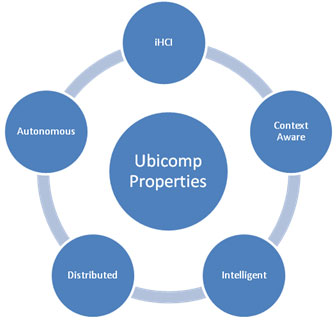
\includegraphics[width=0.5\linewidth]{Images/properties.jpg}
    \caption{ Điện toán môi trường xung quanh}
    \label{ubicomp}
\end{figure}

Cụ thể hơn, các công nghệ đang ứng dụng Ubiquitous Computing có thể kể tới như:
\begin{itemize}
    \item Phương tiện tự di chuyển: bằng cách tự động (Autonomous) xác định vị trí và các yếu tố liên quan của nhiều phương tiện và/ hoặc con người (Distributed), hệ thống điện toán môi trường xung quanh có thể nhận diện các đối tượng (con người, vật thể) với nhau (HCI). Sau đó tập trung nhận dạng các yếu tố liên quan (Context Aware), và sau đó có thể tối ưu hoá từng quyết định (Intelligent) của hệ thống.
    \item Nhà thông minh: bằng cách hiểu các thành viên trong nhà đang ở đâu (Distributed), hệ thống có thể tự động hoá thực hiện các tác vụ ở nhà (như mở máy điều hoà, bật đèn, mử cửa,...) tuỳ theo điều kiện thực tế để thuận tiện cho cuộc sống con người.
    \item Chẩn đoán tai nạn: đây là hướng phát triển ứng dụng của điện toán xung quanh được nói đến gần đây. Với những hệ thống "cảm biến" được con người mang theo hằng ngày (điện thoại, đồng hồ thông minh,...) việc nhận diện người đang bị tai nạn đã trở nên dễ dàng hơn.
    \item Chẩn đoán bệnh lý và sức khoẻ tâm thần: đây là ứng dụng của Ubiquitous Computing đang được đẩy mạnh trong giai đoạn hiện nay trong ngành y tế nói chung. Việc tận dụng các hệ thống cảm biến, camera xung quanh con người và những hệ thống đo lường dữ liệu của cá thể (điện thoại, máy tính bảng, đồng hồ thông minh,...) việc cảnh báo sớm nguy cơ mắc bệnh và nhận diện hành vi và sức khoẻ tâm thần của con người dần trở nên khả thi hơn.
\end{itemize}
Vì vậy có thể thấy công nghệ điện toán môi trường xung quanh đã được phổ biến ở thời điểm hiện tại, song khả năng tích hợp và tận dụng các tài nguyên này vẫn còn đang bị hạn chế.

\section{Tổng quan về học máy và trí tuệ nhân tạo giải thích}
Trong cuộc sống hiện đại, trí tuệ nhân tạo ngày càng được phát triển và ứng dụng trong thực tế. Theo sự phát triển của thế giới, trí tuệ nhân tạo ngày càng được tối ưu và có được khả năng hiểu và phân tích một cách logic. Sự phát triển này của trí tuệ nhân tạo ngày càng thúc đẩy sự phát triển của con người dẫn tới một viễn cảnh con người và máy có thể kết hợp thực hiện các việc con người chưa từng nghĩ là có thể.
\subsection{Lịch sử học máy}
Học máy, một nhánh của trí tuệ nhân tạo, ra đời với khát vọng tạo ra những hệ thống có khả năng học hỏi và tự cải thiện từ dữ liệu, giúp con người giải quyết được những vấn đề học búa. Ý tưởng này bắt nguồn từ mong muốn mô phỏng quá trình học tập của con người, nơi chúng ta rút ra bài học từ kinh nghiệm để đưa ra quyết định. Những năm 1950 đánh dấu bước khởi đầu khi các nhà khoa học bắt đầu nghiên cứu các thuật toán đơn giản (SVM, cây quyết định) cho phép máy tính nhận biết các mẫu trong dữ liệu. Tuy nhiên, do hạn chế về công suất tính toán và dung lượng dữ liệu, sự phát triển của học máy thời kỳ này còn khá khiêm tốn.

Sau một giai đoạn trầm lắng, học máy chứng kiến sự bùng nổ mạnh mẽ vào đầu thế kỷ 21. Sự gia tăng dữ liệu khổng lồ từ Internet và các thiết bị di động, cùng với sự phát triển của sức mạnh và tài nguyên tính toán, đã tạo điều kiện thuận lợi cho những đột phá trong lĩnh vực này. Các thuật toán học sâu (deep learning) dựa trên mạng thần kinh nhân tạo đã đạt được những thành công vượt trội trong nhiều lĩnh vực, từ nhận dạng hình ảnh đến xử lý ngôn ngữ tự nhiên, và đến giải thích được các sự vật hiện tượng trong cuộc sống của con người. Sự thành công của các ứng dụng học máy trong cuộc sống hàng ngày, như trợ lý ảo, xe tự lái, đã thúc đẩy sự đầu tư mạnh mẽ vào nghiên cứu và phát triển.

Do những điểm ưu việt của học máy đem lại, con người đã bước vào một kỷ nguyên mới, nơi mà con người có thể thu thập những phản hồi và gợi ý từ các hệ thống thông minh. những gợi ý và báo cáo này không những giúp con người kiểm soát được cuộc sống mình tốt hơn mà còn mở ra nhiều vùng đất mới cho con người khám phá về bản thân (như nhu cầu hiểu về bản thân, quản lý năng suất của bản thân,...)
% concept ML

\subsection{Học máy có giám sát}
Học máy có giám sát là một nhánh của trí tuệ nhân tạo, nơi các mô hình máy học được huấn luyện trên một tập dữ liệu lớn, mỗi dữ liệu đều được gắn một nhãn cụ thể. Giống như một đứa trẻ học hỏi từ những ví dụ thực tế, các mô hình này sẽ dần rút ra các quy luật, mối quan hệ giữa dữ liệu và nhãn để có thể đưa ra dự đoán chính xác cho dữ liệu mới.

Để thực hiện quá trình học và dự đoán, nhiều thuật toán khác nhau đã được phát triển có thể kể đến như: XGBoost, Random Forest và SVM.

Cụ thể hơn, XGBoost (hay Gradient Boosting)(tham khảo \cite{xgb,xgbNVIDIA}  và Hình \ref{XGBoost}) là một thuật toán mạnh mẽ, kết hợp nhiều mô hình đơn giản để tạo thành một mô hình phức tạp hơn. Nó có khả năng xử lý dữ liệu lớn và đạt được độ chính xác cao. Random Forest (tham khảo \cite{rf,rf_NVIDIA} và Hình \ref{rfNVIDIA}), cũng là một thuật toán tập hợp (hay Bagging), tạo ra nhiều cây quyết định khác nhau, sau đó kết hợp kết quả của chúng để đưa ra quyết định cuối cùng. Random Forest có khả năng giảm thiểu quá khớp và rất ổn định. Hơn thế, một thuật toán khác SVM, hay Support Vector Machine, tìm kiếm một đường phân cách tối ưu để phân loại dữ liệu. Nó thường được sử dụng khi dữ liệu có thể phân tách tuyến tính.
\begin{figure}[!ht]
    \centering
    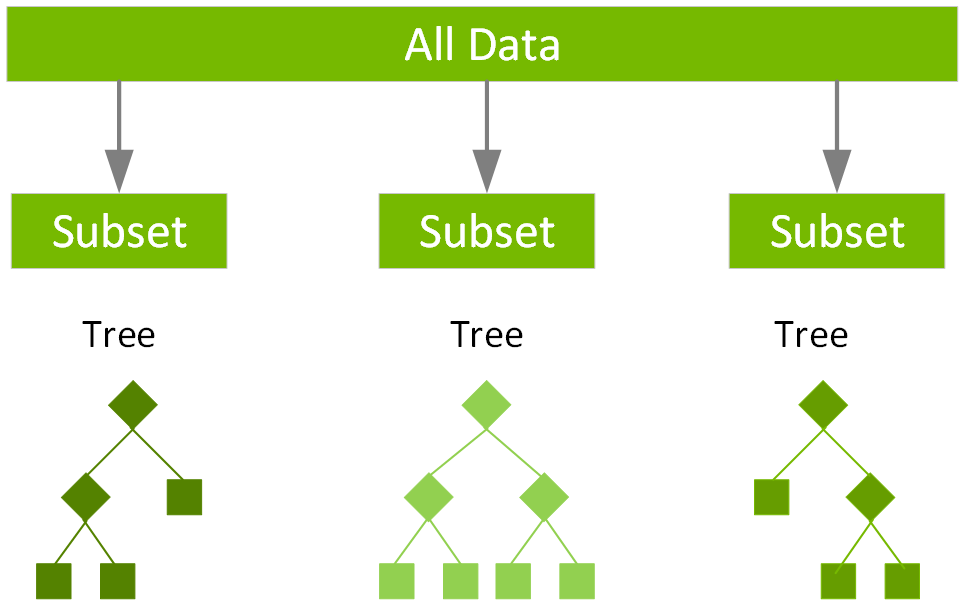
\includegraphics[width=0.8\linewidth]{XGboost.png}
    \caption{Hình ảnh minh hoạ cách phân cây quyết định của XGBoost (Nguồn NVIDA, \cite{xgbNVIDIA})}
    \label{XGBoost}
\end{figure}
\begin{figure}
    \centering
    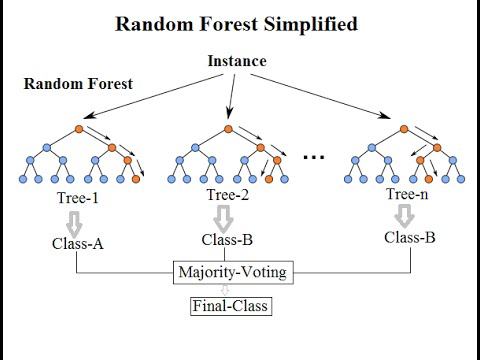
\includegraphics[width=0.8\linewidth]{rf.png}
    \caption{Hình ảnh minh hoạ cách phân cây quyết định của Random Forest (Nguồn NVIDA, \cite{rf_NVIDIA})}
    \label{rfNVIDIA}
\end{figure}
\subsection{Học máy không giám sát}
Nếu học máy có giám sát kể trển là quá trình máy tính học cách gán nhãn cho những dữ liệu có nhãn do ta gán sẵn, thì học máy không giám sát lại là một câu chuyện ngược lại. Ở đây, máy tính sẽ tự mình khám phá, tìm kiếm các mẫu ẩn, các cấu trúc tiềm ẩn trong dữ liệu mà không cần bất kỳ nhãn nào.

Một trong những nhiệm vụ phổ biến nhất của học máy không giám sát là clustering, hay còn gọi là phân cụm. Clustering giúp chia dữ liệu thành các nhóm (cụm) sao cho các điểm dữ liệu trong cùng một cụm có sự tương đồng cao, trong khi các điểm dữ liệu thuộc các cụm khác nhau lại khác biệt. việc phân cụm này giúp cho nhà nghiên cứu có thể quan sát rõ hơn cách hành vi của một hoặc nhiều nhóm dữ liệu có sự tương đồng từ đó hiểu hơn về các nhóm dữ liệu.

Về clustering, các thuật toán nổi trội có thể kể đến như kMEANS, DBSCAN, hoặc Gaussian Mixture Models (GMM). các  thuật toán này đã mở ra khả năng cho việc gom cụm dữ liệu phục vụ và phát triển cho ngành học máy nói chung.


\subsection{Học máy tăng cường}
Nếu ví học giám sát là máy được học dữ liệu qua nhãn dán sẵn, học không giám sát là máy tự tìm ra đặc trưng và gom cụm các dữ liệu có tính tương đồng, thì học tăng cường lại giống như phép thử và làm lại. Nói cách khác, mô hình học tăng cường không chỉ đơn thuần phân loại hay tìm kiếm các mẫu ẩn mà còn tương tác trực tiếp với môi trường. Mô hình sẽ thực hiện các hành động và nhận lại phần thưởng hoặc hình phạt (thông qua hàm nhận và giá cả (gain and loss function)) dựa trên kết quả của hành động đó. Qua quá trình thử và sai liên tục, mô hình sẽ học cách đưa ra những quyết định tối ưu để đạt được mục tiêu đã đặt ra.

\subsection{Học sâu}
khi nhắc tới học máy hiện đại, học sâu (hay Deep Learning) lấy được sự chú ý trong thời điểm gần đây. Lấy cảm hứng từ cấu trúc và chức năng của não người, mạng học sâu đã tạo và sử dụng các mạng thần kinh nhân tạo với nhiều lớp để học từ dữ liệu, tìm ra các đặc trưng phức tạp và đưa ra quyết định.

Với học sâu, mạng này có thể tạo thực hiện những công việc từ phân loại (CNN, RNN), gom cụm (NN-clustering) và cũng có thể học tăng cường (Deep Q-Networks (DQN)). Ngoài ra, học sâu còn có một khả năng ưu việt khác là trích xuất dữ liệu - một điều các giải thuật học máy thông thường không thể.

Vì vậy học sâu đang ngày càng mở rộng tầm ảnh hưởng trong thực tế và là công cụ được tin dùng hàng đầu trong kỷ nguyên này.

\subsection{Trí tuệ nhân tạo giải thích}
XAI (Explainable Artificial Intelligence) hay Trí tuệ nhân tạo có thể giải thích là một lĩnh vực nghiên cứu tập trung vào việc làm cho các hệ thống trí tuệ nhân tạo trở nên minh bạch và dễ hiểu hơn. Thay vì chỉ cung cấp kết quả cuối cùng, XAI cho phép chúng ta hiểu rõ quá trình ra quyết định bên trong của các mô hình AI. Điều này đặc biệt quan trọng đối với các hệ thống AI được sử dụng trong các lĩnh vực có liên quan đến an toàn, pháp lý và y tế, nơi mà sự tin tưởng vào các quyết định của AI là vô cùng cần thiết. XAI sử dụng nhiều kỹ thuật khác nhau để giải thích, từ việc đơn giản hóa các mô hình phức tạp đến việc tạo ra các bản trực quan hoá về cách các yếu tố đầu vào ảnh hưởng đến kết quả cuối cùng.

XAI mang đến nhiều ứng dụng thực tế quan trọng, đặc biệt trong việc giải thích các quyết định phức tạp của các mô hình AI. Như trong lĩnh vực tâm lý học, XAI có thể được sử dụng để giải thích tại sao một mô hình AI lại dự đoán một người nào đó có xu hướng mắc rối loạn tâm lý, hoặc trầm cảm, hay stress. Điều này giúp các nhà tâm lý học hiểu rõ hơn về quá trình ra quyết định của mô hình và từ đó đưa ra những đánh giá chính xác hơn về tình trạng của bệnh nhân. Ngoài ra, trong lĩnh vực thị giác máy tính (Computer Vision), XAI có thể được dùng để giải thích tại sao một mô hình lại xác định một vật thể trong hình ảnh là một con mèo chứ không phải một con chó, một khối u là lành tính chứ không phải ác tính,... Bằng cách làm rõ những yếu tố hình ảnh quan trọng mà mô hình dựa vào, chúng ta có thể đánh giá được độ tin cậy của kết quả và cải thiện hiệu suất của mô hình.

Do vậy XAI đang nổi lên như là một phương pháp hiện đại trong ngành kỹ thuật y sinh - nơi những kết quả cần có những lý giải chính xác cũng như những lý giải đó sẽ giúp con người có cái nhìn tổng quan về cuộc sống của chính bản thân mình.
\begin{figure}
    \centering
    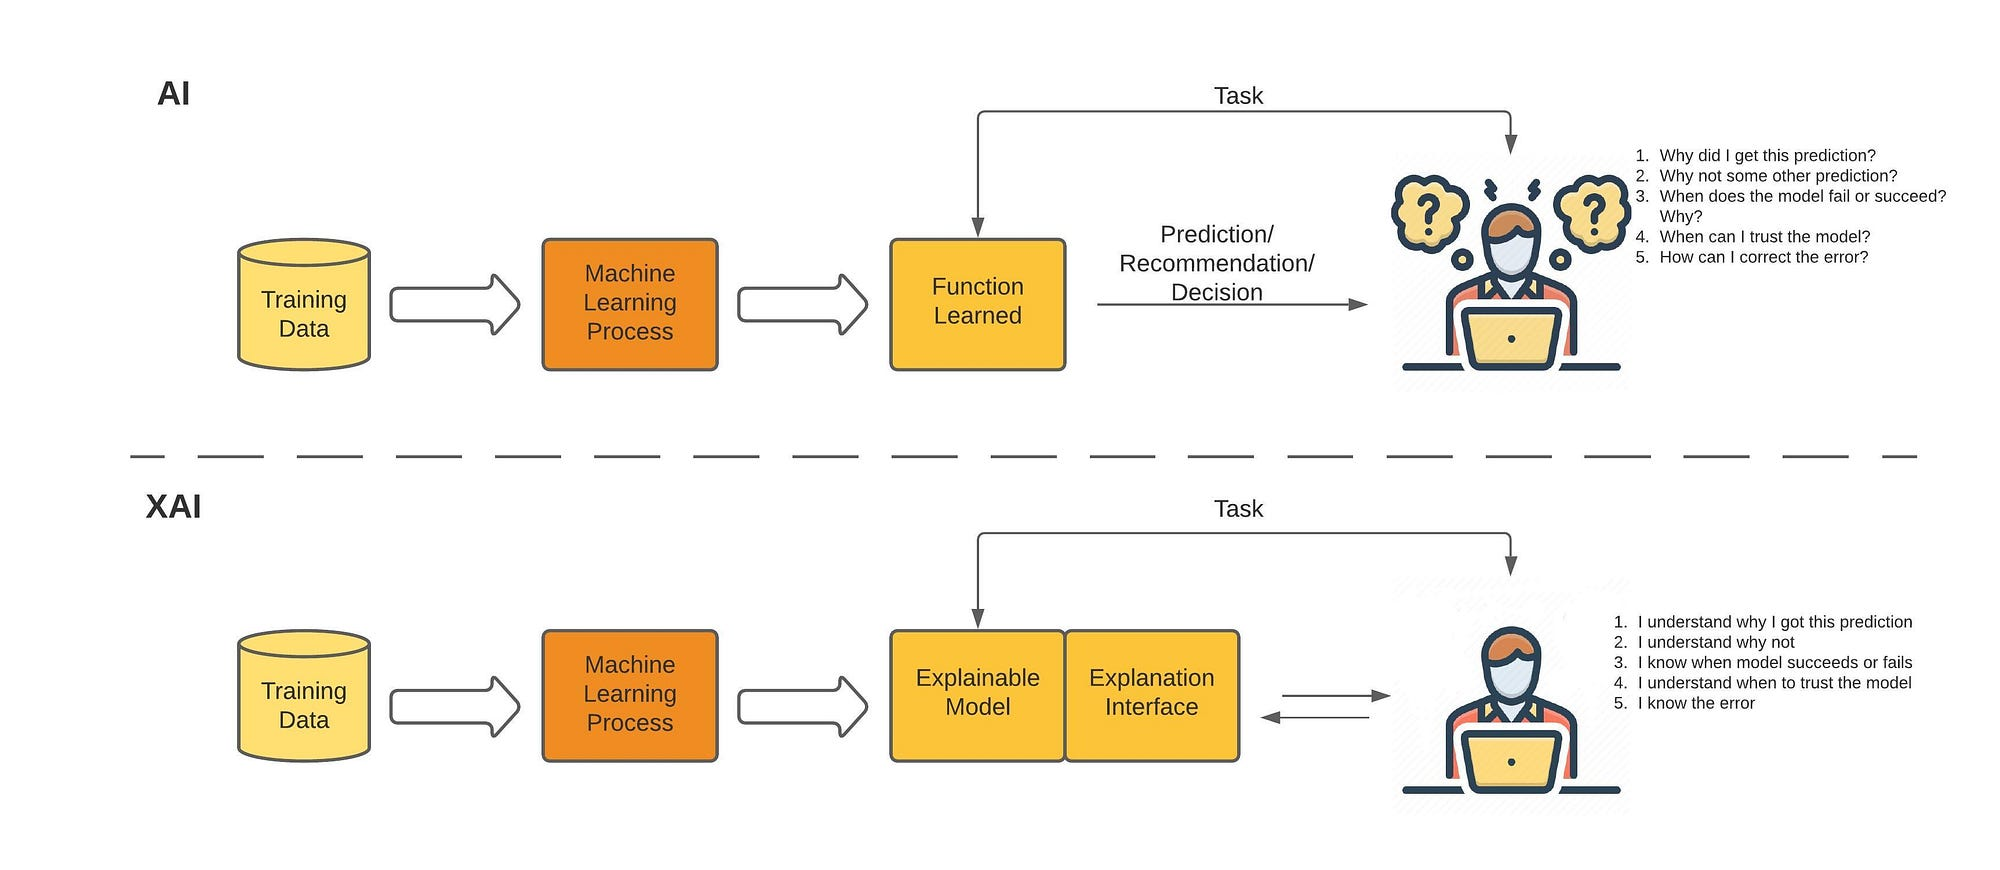
\includegraphics[width=\linewidth]{XAI.jpeg}
    \caption[]{So sánh cách hoạt động của mô hình AI truyền thống (trên) và XAI (dưới) (Nguồn Medium\footnotemark)}
    \label{fig:enter-label}
\end{figure}
\footnotetext{Understanding XAI and EBM truy cập từ: https://medium.com/predmatic/understanding-xai-and-ebm-112bcc7babc3}
\newpage
\section{Các nghiên cứu liên quan}
Căng thẳng tâm lý và tác động của căng thẳng tâm lý là một đề tài được quan tâm từ giới nghiên cứu  \cite{stress_heartrate,Stress_thermo,stress_eeg,student_life,student_life2,student_life3,student_life4,eustress_distress,eustress_distress2,eustress_distress3,eustress_distress4}. Với sự phát triển này, các vấn đề tâm lý đang có thể nhận diện bằng nhiều nguồn khác nhau: tín hiệu y sinh \cite{stress_eeg,stress_eeg2, stress_heartrate}, camera \cite{Stress_thermo}, tín hiệu điện thoại \cite{student_life, student_life2}. Việc này càng đẩy mạnh sự phát triển của công nghệ nhận diện sức khoẻ tinh thần, đưa ra những phương pháp nhận diện sức khoẻ tinh thần đáng tin cậy.
% add table of 
\subsection{Các nghiên cứu không sử sử dụng thiết bị di động}
NhTrong nhận diện sức khoẻ tinh thần, các tín hiệu y sinh là điều quan trọng để nhận diện được tình trạng tâm  lý của một đối tượng. Vì vậy nhóm nghiên cứu của Houtan \cite{stress_eeg} đã thực hiện đo tín hiệu điện não (EEG) của 11 tình nguyên viên trong công trường. Sử dụng các đặc trưng từ tín hiệu EEG theo miền thời gian, và miền tần số nghiên cứu này đã đạt được mô hình phân loại với độ chính xác cao (từ 60\% đến 80\%). Nhưng nhóm nghiên cứu này đề cập về vấn đề của sư suy giảm sư chính xác của việc nhân diên các diễn biến của tâm lý liên tục thông qua cửa sổ trươt (sliding window).

Về các nghiên cứu sử dụng tín hiệu y sinh, Salai và các cộng sự đã ứng dụng cảm biến nhịp tim đã có thể tạo ra mô hình phân loại stress tâm lý trên 46 tình nguyện viên với độ chính xác 75\% \cite{stress_heartrate}. Với mô hình này, nhóm của Salai sử dụng các yếu tố nhịp tim cổ điển như giá trị độ lệch chuẩn nhịp tim trung bình, nhịp tim trung bình, căn bậc hai trung bình của các chênh lệch liên tiếp (RMSSD) và PNN50 để làm đặc trưng của mô hình phân loại.

Về nghiên cứu dùng tín hiệu nhiệt hồng ngoại, Xiao và nhóm của mình đã thực hiện nghiên cứu trên tập dữ liệu bao gồm 32 sinh viên và học viên cao học \cite{Stress_thermo} trong môi trường có kiểm soát. Với ý tưởng stress sẽ gây tác động lên cơ thể, kích thích hệ thần kinh thực vật tạo phản ứng sinh mồ hôi và sẽ làm giảm cường độ hồng ngoại, nhóm đã tận dụng yếu tố sinh học này để thu thập các tín hiệu hồng ngoại này. Sau đó khi đưa các tín hiệu đầu vào này vào mô hình phân loại (Resnet) nhóm thu được kết quả khi chỉ sử dụng tín hiệu hồng ngoại độ chính xác của mô hình lên đến 76\%.

\subsection{Các nghiên cứu sử dụng thiết bị di động}
Để vượt qua các khó khăn về mặt nhận diện stress hằng ngày, các nhóm nghiên cứu \cite{student_life,student_life2,Muller,student_life4} đã đưa ra các cách để thu thập và nhận diện stress tâm lý trong tự nhiên có thể kể đến cụ thể như nhóm của Wang với đề tài StudentLife \cite{student_life}. Với dự án này nhóm đã thực hiện nghiên cứu trên 48 sinh viên tại đại học Dartmouth (Dartmouth College) về hành vi di chuyển thông qua định vị vệ tinh toàn cầu (GPS) và các yếu tố xoay quanh cuộc sống sinh viên. Nghiên cứu của nhóm gợi ý những đặc trưng về vị ví và ứng dụng mô hình cây quyết định để đánh giá các yếu tố về tâm lý cũng như học tập của sinh viên. Nghiên cứu này của Rui Wang chỉ ra rằng có thể giảm đến 63\% số lượng đặc trưng và đẩy nhanh tốc độ mô hình bằng việc chỉ xem xét các yếu tố được gợi ý của nhóm.

Vào năm 2022, nhóm của Wang phát triển trên hệ thống StudentLife khảo sát sự khác biệt của hành vi của sinh viên năm 1 và sinh viên các năm còn lại \cite{student_life4}. Ở nghiên cứu này, các đặc trưng về hoạt động thể chất, vị trí (bao gồm thời gian ở trong phòng ký túc xá cá nhân, ký túc xá của người khác, thời gian ở nhà ăn, tổng số địa điểm đến trong ngày,...), thời lượng sử dụng điện thoại, chất lượng giấc ngủ, và tính lặp lại của các đặc trưng được khảo sát kỹ. Về kết quả, nghiên cứu này chỉ ra được nhiều điểm khác biệt về hành vi của các sinh viên năm 1 với các sinh viên năm khác như: mức độ trầm cảm, mức độ stress, sự tham gia lớp học của sinh viên năm đầu và những sinh viên còn lại. Nghiên cứu này cũng chỉ ra rằng thời gian ở Greek house (một dạng nhà văn hoá dành cho sinh viên) và thời gian ở phòng ký túc xá của cá nhân là những thời gian quan trọng ảnh hưởng đến sức khoẻ tinh thần của sinh viên. Thế nhưng một hạn chế của nghiên cứu này là chưa thể hiện được lượng hoá được độ quan trọng của tất cả đặc trưng trích xuất, và chưa thể giải thích được lý do stress của từng sinh viên.

Một cách tiếp cận phát triển nghiên cứu \cite{student_life4} được nhóm của Muller đề xuất \cite{Muller} bằng cách xem xét thời gian ở nhà, số địa điểm đến, tổng quãng đường di chuyển, thời gian ở các địa điểm quan trọng, và thời gian di chuyển. Nhóm của Muller kết luận được thời gian ở nhà, và số địa điểm đến trong ngày mang ý nghĩa quan trọng đến sức khoẻ tinh thần. Hơn thế, nhóm cũng nêu lên sự cần thiết về việc hiểu các tác động của từng yếu tố lên sức khoẻ tinh thần của con người. Ngoài ra, bài nghiên cứu này cũng tập trung vào xu hướng di chuyển. Với việc khám phá xu hướng di chuyển, việc tìm ra các xu hướng của hành vi này sẽ giúp ta có thể kết nối sức khoẻ tinh thần và hành vi của con người.

Vào năm 2023, một nhóm nghiên cứu do Xu dẫn đầu đã phát triển từ mô hình của Wang, đã đưa lên một bộ dữ liệu là kết quả của sự kết hợp của 2 bộ dữ liệu về trầm cảm hiện có, đặt ra vấn đề mở rộng chủng tộc và đặt thách thức cho một hệ thồng toàn diện cho việc nhận diện stress\cite{student_life2}. Ở nghiên cứu này, nhóm xem xét các yếu tố vị trí, hoạt động điện thoại, di chuyển,... ở các buổi - điều các nghiên cứu trước chưa có nhiều sự quan tâm - để tìm ra đặc trưng dữ liệu. Về kết quả, nhóm đã đạt được độ chính xác phân loại stress vào khoảng 58\%, một sự phát triển đáng kể so với các nghiên cứu trước.


% Vào năm 2024, một nghiên cứu về tâm lý khác đã được thực hiện bởi Nepal thực hiện trong vòng 4 năm để nhận diện các vấn đề tâm lý của sinh viên đại học trước và sau COVID 19 \cite{student life3}. Nghiên cứu này đã chỉ ra được các sự khác biệt trong hành vi con người trước và sau đại dịch và gợi ý phương hướng cho các nghiên cứu thực hiện thu thập dữ liệu của người dùng để phát hiện cá trạng thái và đưa ra những ứng xử phù hợp

\subsection{Nghiên cứu ứng dụng trí tuệ nhân tạo giải thích}
Việc ứng dụng trí tuệ nhân tạo giải thích trong lĩnh vực tâm lý chưa được quá chú trọng. Song trong lĩnh vực nhận diện và giải thích căng thẳng, nhóm của Shikha \cite{Shikha} đã ứng dụng công nghệ này để giải thích cho mô hình phân loại của nhóm. Ở nghiên cứu này, 58 tín hiệu sinh học được sử dụng để chẩn đoán stress tâm lý. Bằng việc ứng dụng XAI, nghiên cứu này chỉ ra được XAI có khả năng giải thích tốt các đặc trưng thu thập được. 

\begin{longtable}{p{0.05\linewidth}  p{0.25\linewidth} p{0.3\linewidth} p{0.3\linewidth}}

\caption{Bảng biểu về tổng hợp các nghiên cứu liên quan}
\label{related_ửoks_summary_tab}
% \renewcommand{\arraystretch}{1.5}
\fontsize{13}{16}
\selectfont

\hline
 \textbf{ID} &\textbf{Tên công trình}  &\textbf{Phương pháp nghiên cứu}  & \textbf{Kết quả nghiên cứu} \\
\hline
\endfirsthead

\multicolumn{4}{c}%
{{\bfseries \tablename\ \thetable{} -- tiếp theo}} \\
\hline 
 \textbf{ID} &\textbf{Tên công trình}  &\textbf{Phương pháp nghiên cứu}  & \textbf{Kết quả nghiên cứu} \\
\hline 
\endhead
\hline
 \multicolumn{4}{r}{{Tiếp tục ở trang kế tiếp}} \\ 
\endfoot
\endlastfoot
\cite{stress_eeg}&EEG-based workers' stress recognition at construction sites& Thu thập tín hiệu EEG và biển đổi tín hiệu này theo miền thời gian và miền tần số& Mô hình phân loại có độ chính xác cao nhưng vẫn có những thách thức với việc nhận diện ở phương pháp cửa sổ trượt  \\
\cite{stress_heartrate} & Low-cost heart
rate sensor and mental stress detection using machine learning & Phân tích các yếu tố nhịp tim như nhịp tim, PP50,... & Độ chính xác mô hình nhận diện căng thẳng đạt 75\%  \\
        \cite{Stress_thermo} & Reading between the heat: Co-teaching body thermal signatures for non-intrusive stress detection & Phân tích biểu đồ quang cận hồng ngoại để nhận diện stress & Mô hình có độ phân loại có độ chính xác 76\%  \\
       \cite{student_life4}  & First-gen lens: Assessing men-
tal health of first-generation students across their first year at college using mobile sensing & Phân tích các yếu tố hành động của sinh viên & Tìm ra được mối liên hệ của các hành động trong ngày và căng thẳng tâm lý  \\
\cite{student_life2}&Globem: Cross-
dataset generalization of longitudinal human behavior modeling.&Nghiên cứu các hoạt động của sinh viên theo buổi& Độ chính xác phân loại được 58\% với mô hình mà nhóm công bố. So sánh thông số này với các nghiên cứu khác tại thời điểm đó.\\
\cite{Shikha}&Optimization of wearable
biosensor data for stress classification using machine learning and explainable ai& Thu thập các tín hiệu EDA, BVP, IBI sau đó lựa chọn các đặc trưng theo chiến thuật Thuật toán di truyền với thông tin tương hỗ (GA-MI) \cite{GAMI} để chọn đặc trưng sau đó huấn luyện và giải thích mô hình bằng XAI& Chứng minh XAI có thể giải thích mô quyết định của mô hình tương đối chính xác với thực tế và các công cụ thống kê khác.




\hline
% \textbf{class\_schedule} & The time student have to go to school in that day\\
% \hline
% \multicolumn{2}{l}{$^*$ The total time is calculated by $\sum_{i\subset S} \{time\ diffence\}_i$, and the std is calculated by $\sum_{i\subset S} \{time\ diffence\}_i$ with 
% }\\
% \multicolumn{2}{l}{S is the set of grouped features in a day}

\label{feature_type}

\end{longtable}
% (to be added more papers in this group :( )


% Do khả năng tinh chỉnh cục bộ và đưa ra giải thích cục bộ, LIME phù hợp với việc giải thích quyết định của mô hình nhận diện stress do khả năng xem xét 





\newpage
\chapter{Phương pháp nghiên cứu}
Trong nghiên cứu này, tôi đã trích xuất các đặc trưng dựa trên thời gian, dựa trên lịch học tập, vị trí, và di chuyển. Đầu tiên, các đặc trưng dựa trên thời gian, bao gồm ngày trong tuần và tuần, được trích xuất. Tiếp theo, tín hiệu GPS của người tham gia sẽ được mã hóa thành tên và loại địa điểm, và được nhóm thành các loại số liệu dựa trên vị trí dựa trên loại và tên của địa điểm đã được trích xuất trước đó. Tiếp theo, tôi sử dụng lịch học tập của sinh viên để tìm lịch trình các lớp học trong một ngày (lịch học). Sau đó, việc ước tính số buổi học bị học sinh bỏ sẽ được thực hiện bằng cách so sánh lịch học với vị trí của sinh viên. Tiếp theo, các thời hạn nộp bài học tập và thời hạn nộp bài học tập sắp tới của sinh viên được trích xuất. Sau đó, bộ dữ liệu được chia thành tập huấn luyện và tập kiểm thử theo tỷ lệ 7:3. Sau đó, tôi đã huấn luyện và kiểm tra các mô hình học máy đã chọn (Random Forest, XGBoost, SVM). Cuối cùng, SHAP được áp dụng để hiểu tác động của từng yếu tố lên quyết định của mô hình.

\begin{figure}
    \centering
    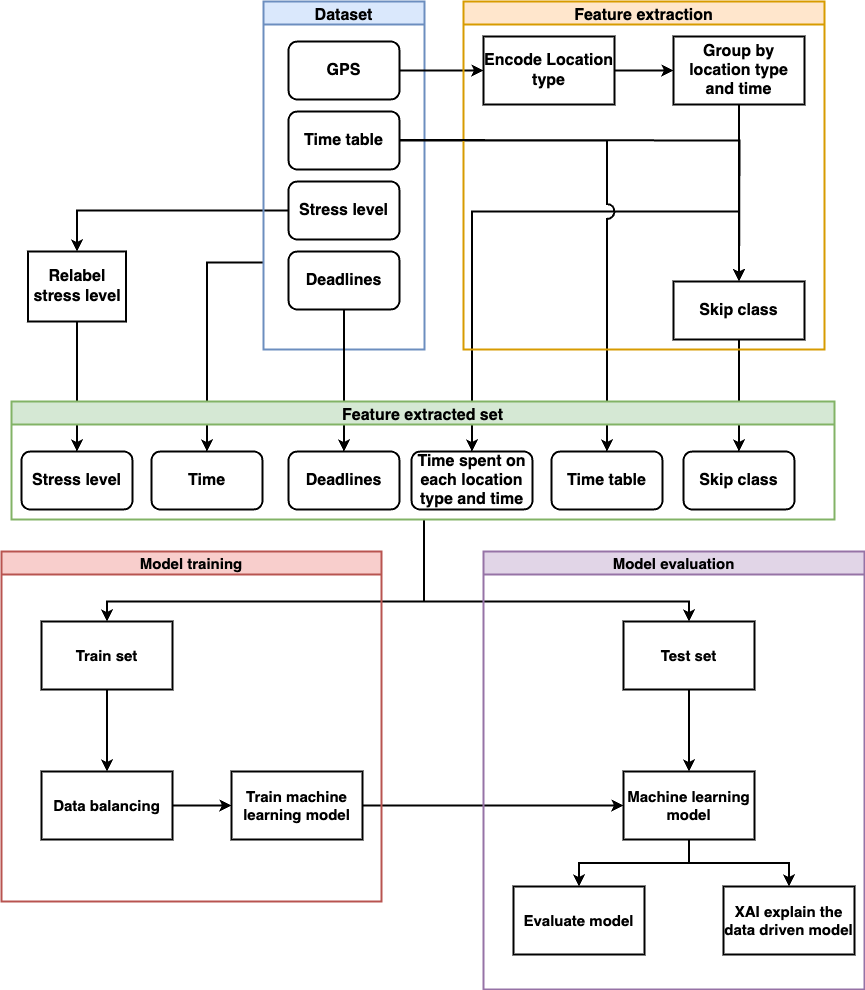
\includegraphics[width=\linewidth]{Images/pipeline_stress.drawio.png}
    \caption{Lưu đồ phương pháp nghiên cứu}
    \label{fig:enter-label}
\end{figure}

\section{Bộ dữ liệu}
Trong nghiên cứu này, bộ dữ liệu StudentLife \cite{student_life} đã được sử dụng để khai thác đặc trưng và phân tích thông tin. Bộ dữ liệu này, được thu thập vào năm 2014, đã sử dụng một ứng dụng Android để theo dõi liên tục nhiều luồng dữ liệu khác nhau bao gồm GPS, nhật ký cuộc trò chuyện, mô hình giấc ngủ và hoạt động ăn uống, bên cạnh việc theo dõi tình trạng sức khỏe tâm thần, sự tham gia lớp học, tâm trạng và hoạt động thể chất của những người tham gia tình nguyện. Bộ dữ liệu bao gồm thông tin từ 48 sinh viên trong một học kỳ 10 tuần tại Đại học Dartmouth. Nghiên cứu này tập trung cụ thể vào việc sử dụng các tập con của bộ dữ liệu, cụ thể là GPS, và thông tin học tập để phân tích và khám phá.

Trong nghiên cứu này, 5 trong số 10 thuộc tính của bộ dữ liệu GPS đã được phân tích (Bảng \ref{dataset}): thời gian, nhà cung cấp, loại mạng, vĩ độ và kinh độ.
\begin{table}[ht]
\caption{Bảng các đặc trưng về GPS được sử dụng và định nghĩa của đặc trưng đó}
\fontsize{13}{16}
\selectfont
\begin{center}
\begin{tabular}{p{0.25\linewidth}  p{0.5\linewidth}}
\hline
\textbf{Đặc trưng}&\textbf{Định nghĩa}\\
\hline
\textbf{Thời gian} & Thời gian trên mốc thời gian Unix khi GPS được thu thập \\

\textbf{Nhà cung cấp} & Nhà cung cấp GPS, là mạng hoặc GPS.\\

\textbf{Loại hình cung cấp} &Loại mạng dùng để thu thập GPS \\

\textbf{Vĩ độ} &Vĩ độ của tín hiệu GPS\\

\textbf{Kinh độ} & Kinh độ của tín hiệu GPS \\
\hline
\end{tabular}
\label{dataset}
\end{center}
\end{table}



\section{Trích xuất đặc trưng}\label{feat_ext}

Theo phương pháp trích xuất và hiểu biết về hành vi, các đặc trưng được chia thành 3 nhóm:
\begin{itemize}
    \item Đặc trưng dựa trên thời gian: Các đặc trưng dựa trên thời gian đóng một vai trò quan trọng trong việc hiểu hành vi của sinh viên, đặc biệt là sức khỏe tinh thần của họ. Các yếu tố như thời điểm trong năm và ngày trong tuần có thể ảnh hưởng sâu sắc đến trạng thái tâm lý của họ, thay đổi theo thời điểm trong học kỳ/thời gian trong kỳ nghỉ.
    \item Đặc trưng dựa trên học tập: Cuộc sống học tập đôi khi có vấn đề như hạn nộp bài và thời gian học tập - điều có thể gây ra căng thẳng. Ví dụ, sinh viên có thể cảm thấy căng thẳng nếu có quá nhiều hạn phải nộp trong một ngày. Do đó, việc khám phá các khía cạnh như vậy có thể khám phá thêm các góc độ của cuộc sống sinh viên.
    \item Đặc trưng dựa trên vị trí: Thời gian và bản chất của thời gian dành cho các vị trí cụ thể có thể ảnh hưởng đáng kể đến sức khỏe tinh thần của họ. Ví dụ, thời gian kéo dài ở địa điểm giải trí có thể liên quan đến mức độ căng thẳng thấp hơn do sự tham gia đều đặn, trong khi dành nhiều thời gian ở nhà và bỏ học có thể cho thấy mức độ căng thẳng tăng cao, đặc biệt là vào cuối năm học.


\end{itemize}
Bốn nhóm đặc trưng này mang đặc trưng về hoạt động và hành vi của sinh viên và sẽ được nhóm theo từng ngày. Yếu tố ngày sẽ được trích xuất thông qua thời gian (trình bày tại Bảng \ref{dataset}) theo hệ thời gian "\#Ngày/\#Tháng/\#Năm".
\begin{table}[ht]
\caption{Bảng đặc trưng trích xuất và số lượng }
\fontsize{13}{16}
\selectfont
\begin{center}
\begin{tabular}{p{0.4\linewidth}  p{0.2\linewidth}}
\hline
\textbf{Đặc trưng}&\textbf{Số lượng}\\
\hline
Đặc trưng thời gian& 2\\

Đặc trưng học tập& 9\\

Đặc trưng vị trí& 39\\

\hline
\end{tabular}
\label{tab1}
\end{center}
\end{table}

\subsection{Đặc trưng thời gian}
Như đã trình bày ở phần \ref{feat_ext} thời gian là một phần rất quan trọng trong cuộc sống sinh viên. nó miêu tả được sự đến gần giữa những kì thi quan trọng trong học kì cũng như nêu lên được tính quá trình trong quá trình học vấn. Vì vậy ở nghiên cứu này tôi đưa ra 2 đặc trưng trong đặc trưng này bao gồm:
\begin{itemize}
    \item Tuần: là tuần trong năm được đánh số từ 1 đến 52. Đặc trưng này sẽ thể hiện tính quá trình trong thời gian học tập. Với lịch học của đại học Dartmouth thời điểm khảo sát (khảo sát từ tuần 12 đến tuần 22), tuần 16 được đánh dấu là tuần thi giữa kì.
    \item Ngày trong tuần: đặc trưng này sẽ xem xét các ngày trong tuần và khảo sát mức độ stress của học sinh tỏng những ngày trong tuần, từ đó đưa ra gợi ý về những ngày mà sinh viên có thể cảm thấy quá sức.
\end{itemize}

Đặc trưng này được trích xuất bằng cách xem xét thời gian (trình bày tại Bảng \ref{dataset}) theo hệ thời gian \#Giờ; \#Phút; \#Giây; \#Ngày; \#Tháng; \#Năm; \#Tuần; \# Thứ;... hoặc là tổ hợp tuỳ ý các yếu tố theo định dạng bất kỳ do người dùng đặt. Việc chuyển đổi này được thực hiện thông qua hàm strftime từ thư viện datetime\cite{datetime_lib}. 

% Về hàm này, giờ, phút, giây sẽ được định nghĩa bởi: 
% \begin{align}
%     Seconds=R(time,60) \\
%     Minute=R(time,3600) \\
%     Hour=R(time, 86400)
% \end{align}
% với R(x,y) là phần dư của phép chia x cho y.
% Về yếu tố ngày tháng năm đầu tiên

% \begin{align}
%     num\_of\_day&=\lceil \frac{time}{86400}\rceil\\
%     year&=\lfloor \frac{num\_of\_day}{365.25}\rfloor+1970\\
%     month&=\lfloor \frac{num\_of\_day-year\times 365.25}{30}\rfloor\\
%     day&=\lfloor num\_of\_day-year\times365.25-\sum_{i=1}^{month} day\_in\_month_i\rfloor
% \end{align}
\subsection{Đặc trưng học tập}
Việc học là một việc phổ biến trong cộng đồng sinh viên. Với việc khảo sát việc học, các áp lực trong quá trình học tập, các khó khăn về thời lượng lên lớp,... sẽ được khảo sát kỹ. Vậy nên việc khảo sát các yếu tố học tập đóng vai trò quan trọng trong việc hiểu hơn về đời sống sinh viên.
\subsubsection{Yếu tố liên hệ với thời gian đi học} \label{time_on_school_related_feature}
Với bộ yếu tố này, tôi khảo sát về 2 yếu tố quan trong trong học vấn là thời lượng lên lớp và sự nghỉ học của sinh viên.

Với thời lượng lên lớp, việc lên lớp nhiều hay ít sẽ có một tác động nhất định lên đến cuộc sống sinh viên. Theo nghiên cứu của Verma \cite{school_time_and_stress} việc học nhiều sẽ có tác động tiêu cực đến sức khoẻ tinh thần của học sinh. Lấy ví dụ cho một sinh viên, nếu sinh viên phải tham dự nhiều tiết học một ngày, thời gian để sinh viên thực hiện các hoạt động thường ngày khác sẽ bị giảm đi, gây hậu quả tăng khả năng bị stress tâm lý của sinh viên. Vì vậy đây là một yếu tố quan trọng để dự đoán sức khoẻ tinh thần của sinh viên cũng như khi tham khảo đầy đủ yếu tố này sẽ gợi ý được khoảng thời lượng hợp lý cho việc lên lớp của sinh viên.

Về vấn đề đi học và nghỉ học đây là một hoạt động diễn ra trên phần đông sinh viên. Nhưng hiện tại việc hiểu rõ nguyên nhân và tác động của hành vi này chưa được khảo sát kỹ. Ở bài nghiên cứu này, việc nghỉ học của sinh viên sẽ được trích xuất bằng cách xem xét thời gian ở trường của sinh viên (xem phần \ref{location_feat}) và phần thời gian lên lớp đã trình bày ở trên. Tỉ số tham gia lớp học sẽ được trích xuất bằng phương trình \eqref{class_attendance_rate}


\begin{equation}
    class\_attendance\_rate=min(\frac{School\_time}{Class\_schedule},1)
    \label{class_attendance_rate}
\end{equation}
Về nghỉ học, nếu tỉ lệ tham gia lớp học nhỏ hơn 0.7 thì sẽ gán cho sinh viên đã nghỉ học trong ngày đó và ngược lại. Với yếu tố nghỉ học này, bài nghiên cứu này sẽ nghiên cứu về tỉ số tham gia lớp học và nghỉ học trong ngày. Riêng yếu tố nghỉ học, yếy tố này sẽ được xem xét đến 3 ngày kể từ ngày nghỉ học để xem trạng thái tâm lý của sinh viên.

Một điểm mới ở nghiên cứu này là sự khám phá về lý do cho sự nghỉ học và căng thẳng tâm lý. Việc đánh mẫu lý do nghỉ học được biểu diễn như(xem mã giả \ref{Skipclassreason}). Nghiên cứu này sẽ khám phá về lý do nghỉ học bao gồm nghỉ học để ở nhà, và nghỉ học đề làm các việc ngoài nhà.

\begin{algorithm}
\fontsize{13}{16}
\selectfont
\caption{Mã giả đánh mẫu lý do nghỉ học của sinh viên}
\label{Skipclassreason}
\begin{algorithmic}
\Require Class attendance rate, home time, school and home off time
\State home time adjust$\gets$ home time-sleep\_time(h)
\If{Class attendance rate >0.7}
\State \Return "Not skip class"
\ElsIf {home time adjust>school and home off time}
\State \Return "Skip class for home purposes"
\Else
\State \Return "Skip class for outdoors reasons"
\EndIf

\end{algorithmic}
\end{algorithm}

Với yếu tố này sẽ làm rõ hơn về các hành động và hành vi của sinh viên trong quá trình học vấn, giúp tạo nên góc nhìn toàn diện hơn vào đời sống của sinh viên.

\subsubsection{Yếu tố ngoài thời gian đi học}
Về yếu tố này, hạn nộp bài được dùng để nghiên cứu mối liên hệ giữa hạn nộp và stress tâm lý của sinh viên. Dễ thấy được ràng nếu sinh viên có nhiều việc và nhiều thời hạn nộp bài đến gần, việc phân bổ thời gian cho những thời hạn đó đôi lúc sẽ xuất hiện những vấn đề, và sẽ làm cho sinh viên tâm lý bị tụt lại phía sau những thời hạn. Vậy nên việc nghiên cứu sâu vào đặc trưng này sẽ giúp hiểu cách quản lý thời gian và thời hạn của sinh viên, đưa ra được các gợi ý cho giáo viên về thời gian và phân bố những hạn nộp bài để hạn chế đưa sinh viên của mình vào những tình huống khó.

Với đặc trưng này, bài nghiên cứu sẽ khảo sát từ 3 ngày trước thời hạn đến ngày thời hạn phải nộp bài để xem xét tác động của thời hạn nộp bài đến sức khoẻ tinh thần của sinh viên.

\subsection{Đặc trưng vị trí}\label{location_feat}
Để tuân thủ các cân nhắc về bảo vệ quyền riêng tư của tình nguyện viên, các đặc trưng dựa trên vị trí đã được lấy từ tín hiệu GPS phải được mã hoá và sử dụng mà không tiết lộ tọa độ chính xác. Để đạt được mục đích đó, tôi đã sử dụng dịch vụ API Nominatim. Dịch vụ này giúp dữ liệu kinh độ và vĩ độ đã được chuyển đổi thành loại địa điểm. Với cách tiếp cận này, không chỉ tính hữu dụng của bộ dữ liệu được nâng cao mà còn đảm bảo tính ẩn danh của tình nguyện viên. Việc gán nhãn cho vị trí được thực hiện thông qua mã giả \ref{location_entities}.

\begin{algorithm}
\fontsize{13}{16}
\selectfont
\caption{Mã giả gán vị trí cho từng mẫu}
\label{location_entities}
\begin{algorithmic}
\Require Latitude, Longitude

\State Location\_attributes $\gets$ Nominatim\_respond((Latitude, Longitude))
\State Location\_name $\gets$ Location\_attributes[name]
\State Location\_type $\gets$ Location\_attributes[type]
\State \Return Location\_name and Location\_type
\end{algorithmic}
\end{algorithm}
\begin{longtable}{p{0.2\linewidth}  p{0.25\linewidth} p{0.45\linewidth}}

\caption{Bảng biểu về định nghĩa và ý nghĩa các nhóm vị trí trong đặc trưng vị trí}
\label{feature_type}
% \renewcommand{\arraystretch}{1.5}
\fontsize{13}{16}
\selectfont

\hline
\textbf{Loại hình vị trí}&\textbf{Định nghĩa}& \textbf{Ý nghĩa}\\
\hline
\endfirsthead

\multicolumn{3}{c}%
{{\bfseries \tablename\ \thetable{} -- tiếp theo}} \\
\hline 
\textbf{Loại hình vị trí}&\textbf{Định nghĩa}& \textbf{Ý nghĩa}\\
\hline 
\endhead
\hline
 \multicolumn{3}{r}{{Tiếp tục ở trang kế tiếp}} \\ 
\endfoot
\endlastfoot
\textbf{Nhà} & Những địa điểm sinh viên sử dụng như là nhà như nhà, ký túc xá, chung cư,...& Thời gian sinh viên có thể ở nhà là khoảng thời gian quý báu cho sinh viên, giúp sinh viên có thêm thời gian để thư giãn hoặc hoàn thành các kế hoạch của bản thân \\

\textbf{Trường} & Là những địa điểm trường học như trường học, trường đại học, học viện,...& Đối với sinh viên, thời gian ở trường không những là những giờ lên lớp mà còn trao đổi, trò chuyện về các vấn đề học tập cuộc sống với các bạn xung quanh, từ đó góp phần giúp sinh viên xử lý vấn đề stress. \\

\textbf{Di chuyển} & Những địa điểm dành cho việc đi lại như trạm xe bus, đường xá,...& Việc di chuyển đôi khi gây mệt mỏi cho sinh viên và sự mệt mỏi này có thể lan sang sức khoẻ tâm thần. Vì thế đặc trưng này sẽ thể hiện thời gian sinh viên dùng để di chuyển trong ngày để hiểu hơn về cuộc sống sinh viên \\

\textbf{Mua sắm} & Địa điểm dành cho việc mua sắm bao gồm siêu thị, chợ, tiệm bánh,...& Mua sắm là một phần quan trọng trong cuộc sống, việc đi mua sắm giúp con người tận hưởng các thành quả làm việc của mình, và sự thoả mãn khi chi tiêu cho thứ việc mà con người thích có thể làm giảm sự căng thẳng tâm lý  \\

\textbf{Làm việc} & Địa điểm làm việc như nhà máy, văn phòng,...& Việc làm việc là thứ không thể thiếu đến cuộc sống con người, và đôi khi việc đi làm mang đến nhiều trạng thái tâm lý khác nhau với con người dựa trên mức độ công việc và sự tương tác trong lúc làm việc. Vì thế, thời gian làm việc có thể phản ánh phần nào về hành động và hành vi của sinh viên trong ngày\\

\textbf{Giải trí} & Địa điểm dành cho việc giải trí như nhà sách, quán bar,... & Giải trí là một hoạt động thiết yếu cho con người. Việc rời xa khỏi công việc và có thời gian cho bản thân sẽ giúp cá nhân có một khoảng riêng tư để tự hiểu bản thân mình. Việc thấu hiểu bản thân và có thời gian nghỉ ngơi này sẽ giúp cho con người xử lý được các vấn đề của cá nhân. \\

\textbf{Khác} & Những địa điểm khác & (-) \\
\hline
% \textbf{class\_schedule} & The time student have to go to school in that day\\
% \hline
% \multicolumn{2}{l}{$^*$ The total time is calculated by $\sum_{i\subset S} \{time\ diffence\}_i$, and the std is calculated by $\sum_{i\subset S} \{time\ diffence\}_i$ with 
% }\\
% \multicolumn{2}{l}{S is the set of grouped features in a day}

\label{feature_type}

\end{longtable}



Sau đó, các khoảng thời gian khác biệt giữa các dấu thời gian liên tiếp đã được tính toán để xác định thời gian dành cho các loại địa điểm khác nhau (xem công thức \eqref{time_diff}).
\begin{equation}
    \Delta time= time_i-time_{i-1}
    \label{time_diff}
\end{equation}

Thông tin này sau đó được tổng hợp hàng ngày, nhóm dữ liệu theo ngày để phân tích các mẫu di chuyển của tình nguyện viên.

Thông qua quá trình này, 8 loại địa điểm đã được nhóm lại, như chi tiết trong Bảng \ref{feature_type}, cung cấp những hiểu biết quý giá về sở thích địa điểm hàng ngày và hành vi di chuyển trong khi vẫn bảo vệ quyền riêng tư của cá nhân.

Đặc trưng vị trí sẽ bao gồm tổng thời gian sinh viên dành ra ở các loại vị trí như đã nêu ở Bảng \ref{feature_type} sẽ được trích xuất trong một ngày và theo buổi (buổi sáng từ 6 giờ sáng đến 6 giờ tối và buổi tối trong thời gian còn lại) (chi tiết tại công thức \eqref{total_time_cal}

\begin{equation}
     sum\_time_j=\sum_{i \in S_j}\Delta time_i
    \label{total_time_cal}
\end{equation}
với S là tập những địa điểm thuộc một nhóm đặc trưng j nêu trong bảng \ref{feature_type}

Sau đó để hiểu sự khác biệt của cuộc sống sinh viên ngày và đêm, tôi đề xuất đặc trưng so sánh thời gian ở từng loại vị trí giữa ngày và đêm (xem \eqref{daytimevsnighttime}). Với đặc trưng này, sự sai biệt giữa hoạt động ban ngày và ban đêm sẽ được hiểu rõ từ đó hiểu hơn hành vi của sinh viên.

Cuối cùng số lượng vị trí đến trong ngày sẽ được trích xuất để khảo sát số địa điểm sinh viên đó đến trong ngày. Điều này sẽ làm nổi bật lên việc sinh hoạt của sinh viên là là một tham chiếu với các hoạt động bên ngoài của sinh viên.

\begin{equation}
feature\_time_{day\_vs\_night}=feature\_time_{daytime}-feature\_time_{nighttime}
\label{daytimevsnighttime}
\end{equation}

\section{Đánh dấu mẫu stress}\label{relabel}
Trong bộ dữ liệu StudentLife, nhãn căng thẳng được thu thập ở 5 mức độ: hơi căng thẳng, chắc chắn căng thẳng, căng thẳng nặng, cảm thấy tốt và cảm thấy tuyệt vời, và được dán nhãn từ 1 đến 5 tương ứng.

Vì gán nhãn này không thể hiện được sự đồng biến của cường độ stress và nhãn, tôi quyết định dùng công thức \eqref{relabel_stress} để biến nhãn của căng thẳng có sự đồng biến với độ lớn giá trị của nhãn, cụ thể là cảm thấy tốt và cảm thấy tuyệt vời, hơi căng thẳng, chắc chắn căng thẳng, và căng thẳng nặng sẽ được đánh nhãn mới từ 1 đến 5.
\begin{align}
    \begin{cases}
    label=1 (previous\_label=5)\\
    label=2 (previous\_label=4)\\
    label= previous\_label+2 (\text{trường hợp còn lại})
\end{cases}
\label{relabel_stress}
\end{align}


Tuy nhiên, có thể có một số ngày nhận được nhiều báo cáo, vì vậy đối với những ngày đó, tôi quyết định đánh dấu trạng thái căng thẳng của ngày đó là trần của báo cáo mức độ căng thẳng trung bình. Sau đó, mức độ căng thẳng được dán nhãn lại thành hai trường hợp:
\begin{itemize}
    \item Trường hợp 1 (phân loại 2 lớp):đánh nhãn 1 nếu người đó bị căng thẳng (căng thẳng ít, chắc chắn căng thẳng và căng thẳng), và 0 cho các trạng thái vui vẻ khác. Trong trường hợp này, tỷ lệ phân bố dữ liệu của lớp căng thẳng và vui vẻ là 2400: 350 (xem hình \ref{feat_imb2}).
    \item Trường hợp 2 (phân loại 3 lớp):đánh nhãn 2 nếu người đó bị căng thẳng, 1 nếu người đó bị căng thẳng nhẹ (căng thẳng ít và chắc chắn căng thẳng), và 0 cho các trạng thái vui vẻ. Trong trường hợp này, các bản ghi dữ liệu cho lớp căng thẳng, căng thẳng nhẹ và vui vẻ lần lượt là gần 1800, 600 và 350 (xem hình \ref{feat_imb3}).
\end{itemize}

\begin{figure}[ht]
\subfloat[Trường hợp 1 \label{feat_imb2}]{
    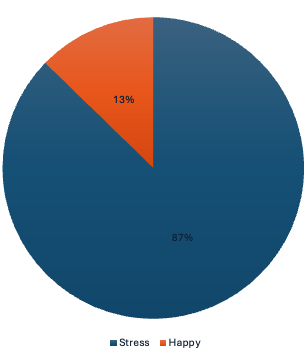
\includegraphics[width=0.45\linewidth]{image.png}
}
% \caption{Random Forest}
% \label{fig_ShaplyRF}
% \end{subfigure}
% \hfill
% \begin{subfigure}[t]{0.24\textwidth}
\subfloat[Trường hợp 2\label{feat_imb3}]{
    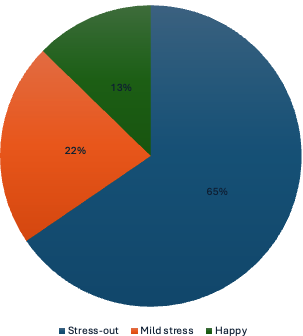
\includegraphics[width=0.45\linewidth]{3class.png}
}
% \caption{XGBoost model}
% \label{fig_ShaplyXG}
% \end{subfigure}
\caption{Sự mất cân bằng dữ liệu trong sự stress của sinh viên ở các trường hợp}
\label{feat_imb}
\end{figure}

\section{Cân bằng hoá dữ liệu}


% \subsection{Phương pháp truyền thống}

Trong nghiên cứu này, một sự kết hợp của các kỹ thuật tăng mẫu và giảm mẫu đã được sử dụng để nâng cao hiệu suất của mô hình phân loại và giải quyết sự mất cân bằng trong phân bố lớp học. Như được minh họa trong Phần \ref{relabel}, sự phân bố không đồng đều của dữ liệu trên các lớp là rõ ràng, với các lớp bị căng thẳng và bị căng thẳng quá mức chiếm hơn 85\% và 65\% dữ liệu huấn luyện trong hai trường hợp, cho thấy sự mất cân bằng đáng kể của dữ liệu stress. Để giảm thiểu vấn đề do sự mấy cân bằng này, sự kết hợp của kỹ thuật tăng mẫu thiểu số tổng hợp (SMOTE) \cite{SMOTE}, với liên kết Tomek \cite{T-links} (đối với trường hợp 2) và hàng xóm gần nhất được chỉnh sửa \cite{ENN} (đối với trường hợp 1) đã được sử dụng. Cách tiếp cận này giúp giảm bớt vấn đề mất cân bằng lớp học và thúc đẩy các dự đoán của mô hình chính xác và đáng tin cậy hơn.

% \subsection{Phương pháp dùng trí tuệ nhân tạo tạo sinh}
% (yet to be done, I have no idea how the model may afect final result, but will try SDV-Gausian Copulas, CopulasGAN, GAN, VAE)
\section{Mô hình huấn luyện}
Trong nghiên cứu này, tôi đã sử dụng ba mô hình học tập tổng hợp, cụ thể là Random Forest, XGBoost và SVM, để dự đoán mức độ căng thẳng hàng ngày bằng cách sử dụng tập đặc trưng đã trích xuất. Để đánh giá hiệu suất của các mô hình này, tôi đã sử dụng xác thực chéo (cross validation) 10 lần, một kỹ thuật được công nhận rộng rãi để đánh giá các thuật toán học máy.
\begin{itemize}
    \item Rừng ngẫu nhiên (RF) là một mô hình học tập, theo hệ số tạp chất Gini kết hợp các cây quyết định và quyết định dựa trên hệ số Gini. Kết quả của mô hình RF là trung bình của kết quả từ các cây quyết định bên trong nó. Nó tổng hợp kết quả từ nhiều cây quyết định để tạo ra một mô hình có độ lệch và phương sai thấp \cite{rf}.
    \item XGBoost là một thư viện tăng cường độ dốc phân tán được tối ưu hóa, được thiết kế để có hiệu quả cao, linh hoạt và di động \cite{xgb}. Nó triển khai các thuật toán học máy theo khung tăng cường độ dốc. XGBoost cung cấp một tăng cường cây song song (còn được gọi là GBDT, GBM) giải quyết nhiều vấn đề khoa học dữ liệu một cách nhanh chóng và chính xác. Cùng một mã chạy trên các môi trường phân tán chính (Hadoop, SGE, MPI) và có thể giải quyết các vấn đề vượt xa hàng tỷ ví dụ.
    \item Máy vectơ hỗ trợ (SVM) là một mô hình học máy cổ điển được thiết kế để tìm kiếm siêu mặt phẳng tối ưu để chia các lớp dữ liệu \cite{SVM}. Do đó, SVM đặc biệt hiệu quả cho các nhiệm vụ để phân biệt 2 hoặc nhiều lớp với độ chính xác cao.
\end{itemize}
Trong quá trình xác thực chéo, bộ dữ liệu được phân chia ngẫu nhiên thành mười tập con, với mỗi tập con đóng vai trò là tập kiểm tra một lần trong khi bốn tập con còn lại được sử dụng để huấn luyện. Quá trình này được lặp lại mười lần, đảm bảo rằng mỗi tập con được sử dụng chính xác một lần làm tập kiểm tra.

Hơn nữa, để đảm bảo tính mạnh mẽ của các đánh giá mô hình của tôi, việc chia tách huấn luyện-kiểm tra được tiến hành ngẫu nhiên giữa tất cả các tình nguyện viên nghiên cứu. Cách tiếp cận này cho phép tôi đánh giá khả năng chung và hiệu quả của các mô hình dự đoán của tôi trên các cá nhân khác nhau trong nhóm tình nguyện viên.

Để đánh giá hiệu suất phân loại của các mô hình của tôi, tôi đã sử dụng mười số liệu đánh giá: độ chính xác, điểm F1 của lớp căng thẳng cao, điểm Weighted F1 và điểm Macro F1. 
Về các số liệu đánh giá, chúng cho phép đánh giá toàn diện hiệu suất của mô hình, xem xét các khía cạnh khác nhau như độ chính xác tổng thể, độ chính xác, độ nhạy và điểm F1, cung cấp một sự hiểu biết sắc thái về hiệu quả của mô hình trong việc phân loại mức độ căng thẳng. Những phân tích thống kê này tạo điều kiện cho việc đánh giá kỹ lưỡng các mô hình của tôi, cho phép tôi đánh giá hiệu quả của chúng và xác định các lĩnh vực cần cải thiện.

\section{Phương pháp đánh giá mô hình}
% Một trong những đánh giá phổ biến trong học máy là báo cáo mô hình phân loại. Trong báo cáo này các đặc trưng (\ref{acc}-\ref{Weighted}) sẽ được sử dụng:
\begin{equation}
    Precision=\frac{TP}{TP+FP}
    \label{P}
\end{equation}
\begin{equation}
    Recall=\frac{TP}{TP+FN}
    \label{R}
\end{equation}
\begin{equation}
    Accuracy=\frac{TP+TN}{TP+TN+FN+FP}
    \label{acc}
\end{equation}
\begin{equation}
    F1=\frac{2\times Precision \times Recall}{Precision+Recall}
    \label{F1}
\end{equation}
\begin{equation}
    Weighted\_F1=\frac{\sum{n_i\times F1_i}}{\sum{n_i}}
    \label{Weighted}
\end{equation}
\begin{equation}
    Macro\_F1=\frac{\sum{F1_i}}{\sum{class}}
    \label{MacroF1}
\end{equation}
với
\begin{itemize}
    \item TP, FP, FN, TN được đề cập trong hình \ref{confmat_img}
    \item $n_i$ là số lượng mẫu hỗ trợ lớp i
    \item $F1_i$ là hệ số F1 (xem công thức \eqref{F1}) của lớp i
\end{itemize} 

\begin{figure}[ht]
    \centering
    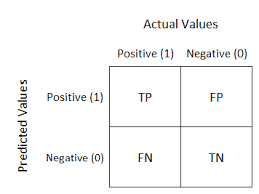
\includegraphics[width=0.5\linewidth]{images-5.png}
    \caption{Hình ảnh trực quan các giá trị trong ma trận nhầm lẫn}
    \label{confmat_img}
\end{figure}

Trong học máy, để đánh giá hiệu suất của một mô hình, độ chính xác \eqref{acc} (accuracy) được sử dụng phổ biến. Giá trị này thể hiện tỷ lệ các dự đoán đúng so với tổng số dự đoán. Độ chính xác thường được chọn làm thước đo đầu tiên bởi tính đơn giản, trực quan và dễ tính toán của nó. Nó cung cấp một cái nhìn tổng quan về hiệu suất chung của mô hình, giúp các nhà nghiên cứu và kỹ sư có thể so sánh hiệu quả giữa các mô hình khác nhau.

Mặc dù vậy, độ chính xác lại có những hạn chế nhất định khi áp dụng cho các tập dữ liệu không cân bằng. Trong trường hợp này, một mô hình có thể đạt được độ chính xác cao đơn giản bằng cách dự đoán tất cả các mẫu vào lớp chiếm đa số. Để khắc phục vấn đề này, các nhà nghiên cứu đã đề xuất sử dụng các thước đo khác, điển hình là weighted F1-score.

Weighted F1-score \eqref{Weighted} là một thước đo tổng hợp, kết hợp cả precision (độ chính xác \eqref{P}) và recall (độ phủ \eqref{R}). Nó tính toán trung bình hài hòa có trọng số của precision và recall, trong đó trọng số của mỗi lớp được điều chỉnh để phản ánh tầm quan trọng tương đối của chúng. Nhờ vậy, weighted F1-score cung cấp một cái nhìn toàn diện hơn về hiệu suất của mô hình, đặc biệt trong các bài toán phân loại có dữ liệu không cân bằng. Việc sử dụng weighted F1-score giúp đảm bảo rằng mô hình không chỉ tập trung vào việc dự đoán chính xác lớp chiếm đa số mà còn chú trọng đến việc phân loại chính xác các lớp thiểu số.

Do những lý do nêu trên, độ chính xác, F1 score lớp stress, và F1 có trọng số sẽ được sử dụng ở bài luận này để đánh giá độ hiệu quả của mô hình.

\section{Phân tích đặc trưng thông qua hệ thống trí tuệ nhân tạo giải thích}
% \subsection{SHAP}
Để hiểu cách mô hình và các đặc trưng đã trích xuất hoạt động, các giá trị SHAPley (SHapley Additive exPlanations) - một công cụ mạnh mẽ để biết được các lý do quyết định của mô hình bằng cách sử dụng lý thuyết trò chơi làm cơ sở để đo lường sự đóng góp của mỗi yếu tố vào mô hình học máy. Nghiên cứu này sử dụng TreeExplainer của khung SHAP để tính toán các giá trị SHAPley (giá trị SHAP) nhanh hơn \cite{tree_explainer} .

Giá trị Shapley là một công cụ mạnh mẽ để đo lường sự đóng góp công bằng của từng người chơi trong một trò chơi hợp tác\cite{shap_value}. Giá trị SHAPley ($\phi_i(x)$) được định nghĩa bởi: 
\begin{equation}
  \phi _i (x) = \sum _{S \subseteq F \setminus \{i\}} \frac{|S|!(|F|-|S|-1)!}{|F|!}[f_{S \cup \{i\}}(x_{S \cup \{i\}})-f_{S }(x_{S })]
\end{equation}  
với:
 \begin{itemize}
   \item $x$: đối tượng quan sát 
   \item $F$: tổng đặc trưng
   \item $f_S$: mô hình huấn luyện trên đặc trưng S
   
   \item $f_{S \cup \{i\}}$: mô hình huấn luyện trên đặc trưng S và i
  \item $x_S$: giới hạn đối tượng quan sát trên miền đặc trưng S
  \item $x_{S \cup \{i\}}$: giới hạn đối tượng quan sát trên miền đặc trưng S và i
 \end{itemize}

Trong lĩnh vực học máy, các đặc trưng đóng vai trò là những người chơi chính quyết định kết quả của mô hình dự đoán, tương tự như những người tham gia trong một trò chơi. Sử dụng các giá trị SHAPley, sự đóng góp của mỗi đặc trưng vào đầu ra của mô hình được làm rõ thông qua các loại biểu đồ khác nhau, hỗ trợ trong việc giải thích hành vi của mô hình.

Một trong những hình ảnh trực quan như vậy, biểu đồ phân tán mật độ, mô tả các giá trị SHAP của mỗi đặc trưng trên tất cả các trường hợp trong tập kiểm tra. Biểu đồ phân tán này cho phép hiểu rõ cách mỗi đặc trưng ảnh hưởng đến các dự đoán của mô hình trên các trường hợp khác nhau. Bằng cách kiểm tra sự phân bố của các giá trị SHAP, chúng ta có thể nhận ra tác động của từng đặc trưng đối với kết quả của mô hình đối với các trường hợp kiểm tra khác nhau.
% \subsection{LIME}
% Một mô hình XAI khác có thể kể tới là LIME \cite{LIME} (Local Interpretable Model-Agnostic Explanations). Với LIME, các yếu tố được quan sát một cách cục bộ, từ đó ta có cái nhìn chi tiết hơn về từng thành phần của mẫu so với SHAP. Và với cái nhìn về từng cá thể của LIME, ta có thể làm bật nên những điểm dữ liệu có tính đặc biệt.

% Về cách thức hoạt động, LIME dựa trên sự biến đổi nhỏ của dữ liệu gốc. Chi tiết hơn, LIME sẽ tạo những phiên bản có sự xê dịch của dữ liệu gốc, sau đó sẽ cho dữ liệu bị xê dịch này vào trong mô hình học máy cần giải thích. Với các xê dịch này sẽ tạo những tạo nên những thay đổi cục bộ mà LIME sẽ dùng để giải thích trên các đặc trưng. Sau đó LIME sẽ đo sức nặng của các yếu tố đặc trưng cục bộ này và sau đó sẽ đưa ra được các giải thích cho từng mẫu quan sát. 
\newpage
\chapter{Kết quả và bàn luận}
\section{Kết quả mô hình phân loại}
\begin{table}[!ht]
\begin{center}

    % \centering
    \caption{Kết quả mô hình phân loại trong 2 trường hợp (đơn vị \%)}
    \fontsize{13}{16}
\selectfont
    \begin{tabular}[10px]{p{0.2\linewidth}| p{0.05\linewidth} p{0.2\linewidth}p{0.05\linewidth}||p{0.05\linewidth}p{0.2\linewidth} p{0.05\linewidth}}
    \hline
    &\multicolumn{3}{l||}{{\textbf{Phân loại 2 lớp}}}&\multicolumn{3}{l}{\textbf{Phân loại 3 lớp}}\\
    \hline
         & $ \hfil$\textbf{XGB} & $ \hfil$\textbf{Random Forest} & $ \hfil$\textbf{SVM} & $ \hfil$\textbf{XGB} & $ \hfil$\textbf{Random Forest}& $ \hfil$\textbf{SVM} \\
         \hline

       \textbf{Accuracy}    & $ \hfil$79& $ \hfil$79& $ \hfil$39 &$ \hfil$65  & $ \hfil$66 &$ \hfil$33 \\

        \textbf{Weighted F1 score}    &$ \hfil$80 &$ \hfil$81 &$ \hfil$45&$ \hfil$61 &$ \hfil$62   &$ \hfil$37 \\

        \textbf{Macro F1 score}   &  $ \hfil$60 & $ \hfil$63 &$ \hfil$37&$ \hfil$45 &$ \hfil$51   &$ \hfil$31\\

         \textbf{F1 score for class stress}     & $ \hfil$88 &   $ \hfil$87&$ \hfil$48 &  $ \hfil$80 & $ \hfil$78&$ \hfil$43 \\  
         \hline
       
         
    \end{tabular}
    
    \label{tab1}


\end{center}
\end{table}
Dựa vào kết quả mô hình phân loại, ta có thể thấy Random Forest có độ chính xác mô hình phân loại tốt nhất với kết quả cho từng tình huống đạt 79\% và 66\%, tốt hơn so với phương pháp nhận diện của Salai, và Xiao \cite{Stress_thermo,stress_heartrate}. Ngoài ra XGB cũng đạt được độ chính xác chấp nhận được khi chỉ thấp hơn Random Forest khoảng 1\% độ chính xác. 

Điểm đặc biệt là ở mô hình SVM. Mô hình này, mặc dù có khả năng phân loại 2 lớp tốt, nhưng sự phức tạp của cuộc sống con người và sự ngẫu nhiên của các hành động và hành vi con người đã gây nhiều nhiễu, làm ảnh hưởng chung đến kết quả của mô hình. 

% Vì vậy ta có thể nhận thấy việc nhận diện hành vi con người thông qua nhận diện vị trí có khả thi trong việc triển khai trong thực tế, song vẫn còn rất nhiều thách thức.
\section{Kết quả phân tích đặc trưng bằng XAI}
\begin{figure}[!ht]
\subfloat[Trường hợp 1 \label{feat_imp2}]{
    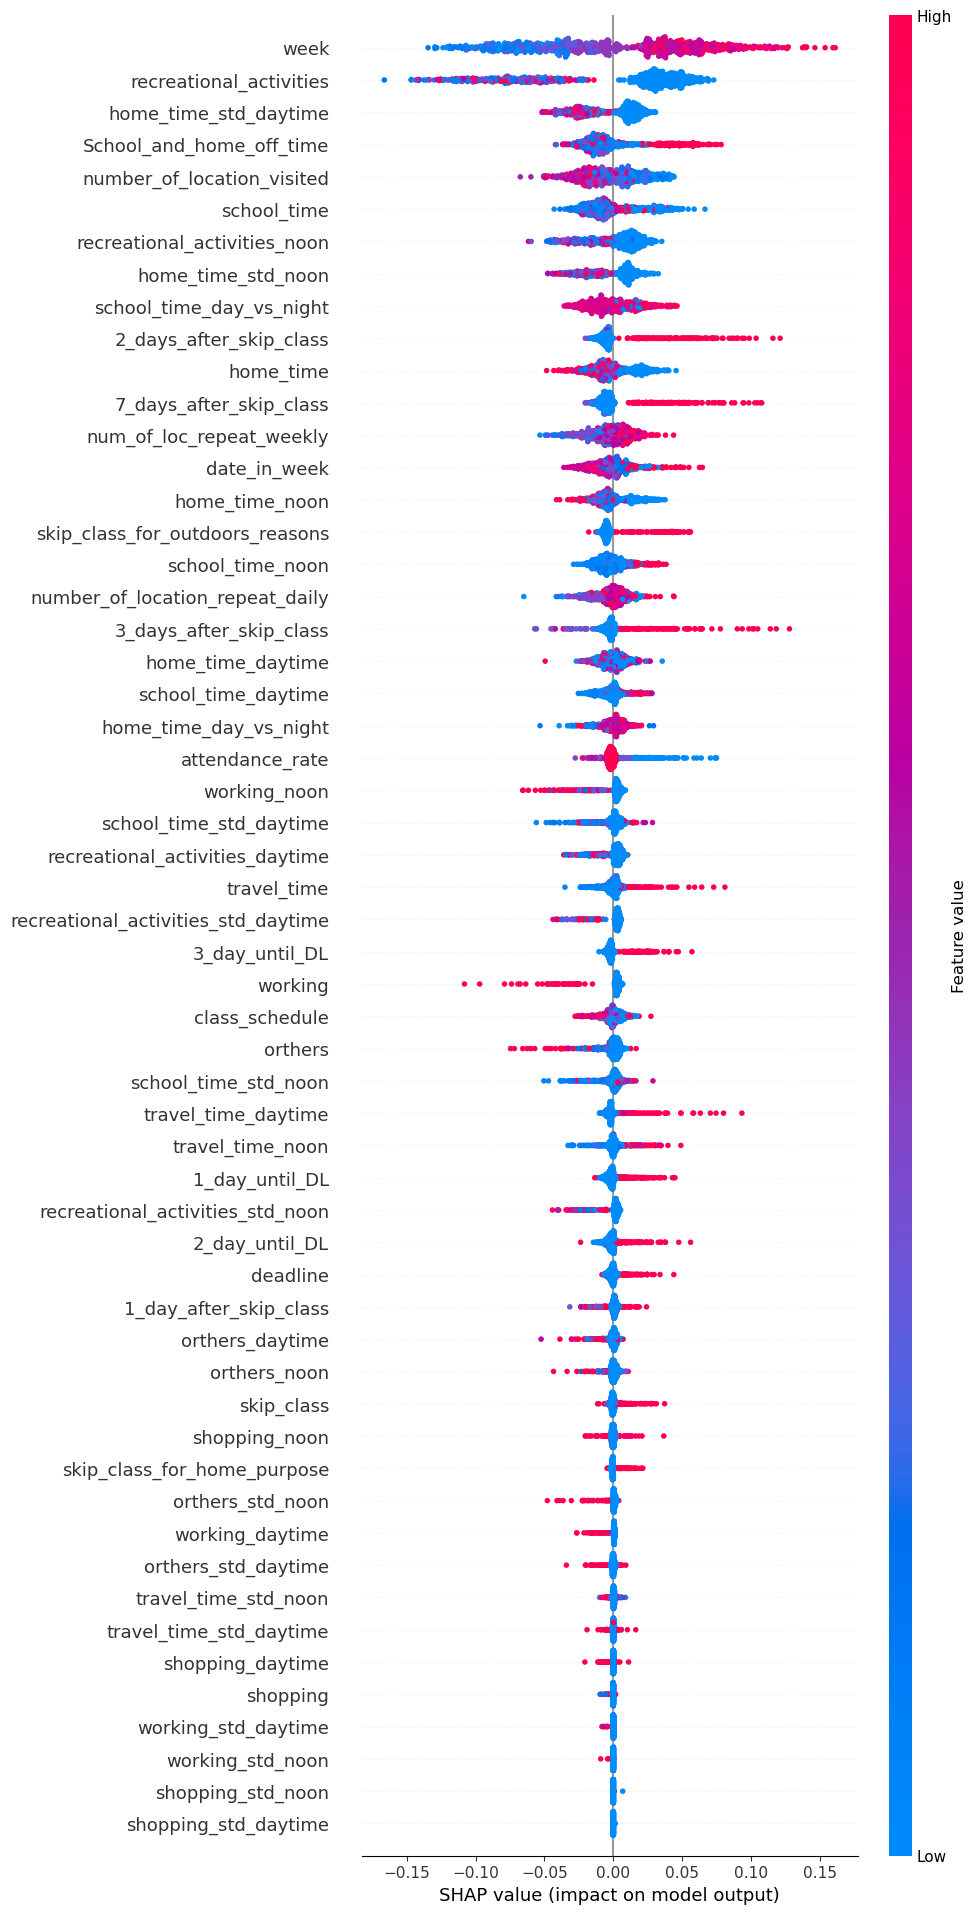
\includegraphics[width=0.45\linewidth,height=0.8\textheight]{Assets/FI_2_class.png}
}
% \caption{Random Forest}
% \label{fig_ShaplyRF}
% \end{subfigure}
% \hfill
% \begin{subfigure}[t]{0.24\textwidth}
\subfloat[Trường hợp 2\label{feat_imp3}]{
    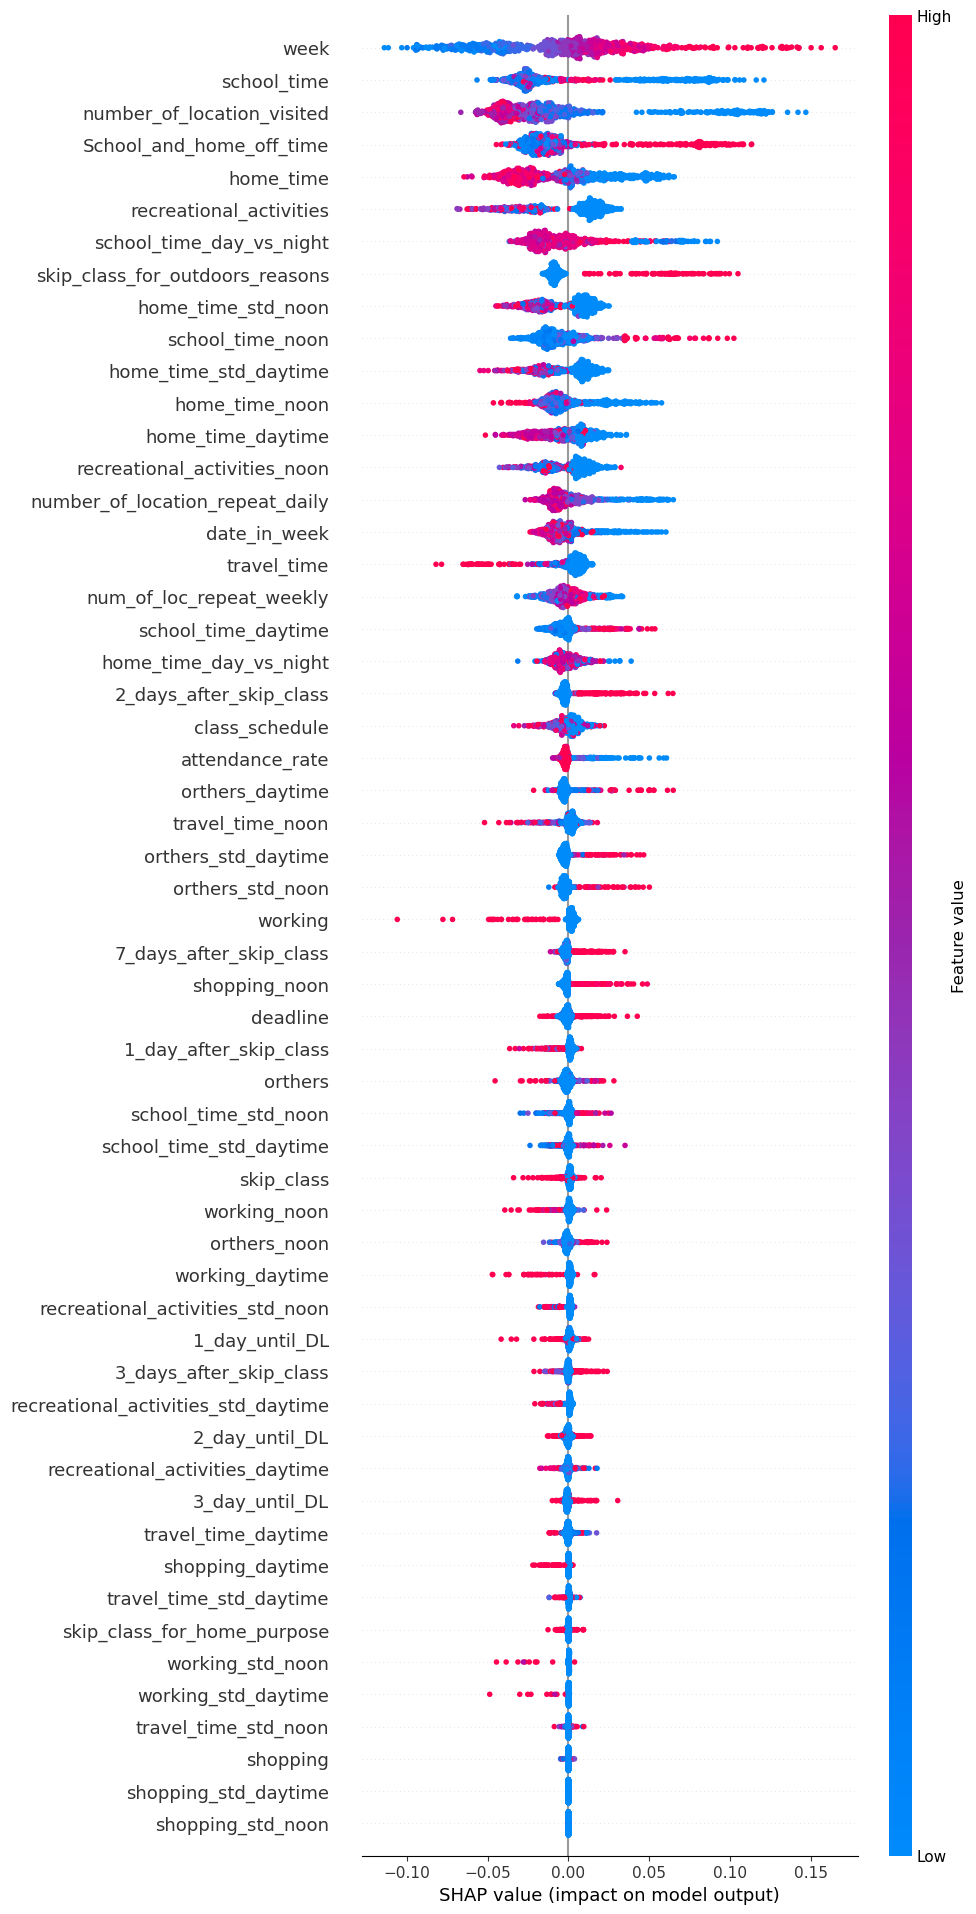
\includegraphics[width=0.45\linewidth,height=0.8\textheight]{Assets/FI_3_class.png}
}
% \caption{XGBoost model}
% \label{fig_ShaplyXG}
% \end{subfigure}
\caption{Biểu đồ phân tích đặc trưng bằng SHAP}
\label{feat_imp}
\end{figure}
% \section{Phân tích SHAP}

Với phân tích SHAP, tuần (week) là yếu tố gây nên căng thẳng tâm lý lớn nhất của sinh viên. Điều này khá dễ hiểu khi việc học diễn ra, càng về sâu của khoá học, lượng kiến thức càng nhiều và nâng cao, dẫn đến người học phải tốn nhiều thời gian hơn để nghiên cứu và hệ thống kiến thức. Điều này vô tình tạo áp lực lên sinh viên và dẫn đến căng thẳng tâm lý.

Một yếu tố khác có thể kể đến là thời gian giải trí (recreational activity) ảnh hưởng lớn đến sức khoẻ tinh thần của sinh viên. Với thời lượng giành cho các hoạt động giải trí cao, sinh viên sẽ có ít khả năng gặp phải các vấn đề tâm lý. Ngoài ra các yếu tố thời gian khác như thời gian ở nhà và ở trường (home time, và school time) cũng có ảnh hưởng lớn đến trạng thái sức khoẻ tinh thần của sinh viên.

Một yếu tố bổ sung mà tôi đã đề cập ở phần \ref{time_on_school_related_feature} là sự nghỉ học đóng góp tốt cho mô hình. Cụ thể hơn, với sinh viên nghỉ học đây có thể là dấu hiệu cho những vấn đề căng thẳng tâm lý, nhưng ngày sau ngày nghỉ học, các vấn đề đó sẽ phần nào được giải quyết (xem hình \ref{feat_imp}). Đây là một vấn đề đáng quan tâm khi là một bằng chứng chứng tỏ việc nghỉ học có thể giúp sinh viên giải quyết được các vấn đề tinh thần.


\section{Bàn luận}
Nghiên cứu này đã đề xuất phương pháp ứng dụng tín hiệu GPS liên tục từ điện thoại sinh viên trích xuất đặc trưng di chuyển và học tập của sinh viên mà vẫn đảm bảo tính bảo mật vị trí trong nghiên cứu sức khoẻ tinh thần dành cho sinh viên với độ chính xác cao (xấp xỉ 80\%) trong môi trường không kiểm soát. Đặc biệt hơn, nghiên cứu này cũng ứng dụng mới nhất trong lĩnh vực trí tuệ nhân tạo - XAI - trong việc khai phá tầm quan trọng của các đặc trưng trích xuất hiểu thêm sâu vào sức khoẻ tinh thần của sinh viên.

Việc phát triển hệ thống nhận diện sức khoẻ tinh thần trong tự nhiên đưa ra những yếu tố định lượng cho việc hiểu về sinh viên của người hoạt động giáo dục. Hơn thế việc có được các dữ liệu này có thể hỗ trợ nhà trường có thêm các cơ sở cho việc sắp xếp thời gian học tập giúp sinh viên có thể cân đối việc học và các việc cá nhân.

Tuy nhiên, nghiên cứu này chỉ có thể sử dụng dạng vị trí (nhà hàng, toà nhà, trường,...) để gán cho loại hoạt động của sinh viên (nhà, trường, giải trí,...). Việc này có thể vô tình gán sai hành động của sinh viên trong thực tế. Vì vậy, tôi đề xuất việc phát triển thêm phương pháp đánh giá hành động của con người hoặc ứng dụng trí tuệ nhân tạo tạo sinh để cải thiện việc hiểu hoạt động này rõ ràng hơn, từ đó chính xác hoá và giải quyết được cấc tình huống phức tạp trong hiện tại ví dụ nhận biết sinh viên đang làm gì trong một toà nhà đa chức năng (ăn uống, mua sắm, học tập).

Ngoài ra, nghiên cứu này đã đề cập các vấn đề liên quan đến vị trí, và hành vi của sinh viên song vẫn chưa hoàn thiện được các yếu tố xoay quanh cuộc sống của sinh viên hiện đại như thói quen tương tác xã hội, thời gian sử dụng điện thoại, học trực tuyến, ... Việc khai phá thêm đặc trưng này sẽ giúp mở rộng những đặc trưng cho việc chẩn đoán sức khoẻ tinh thần của sinh viên cũng như đưa được góc nhìn tổng quát hơn về sinh viên của mình.

\begin{figure}[!ht]
\subfloat[Không nghỉ học \label{feat_imb2}]{
    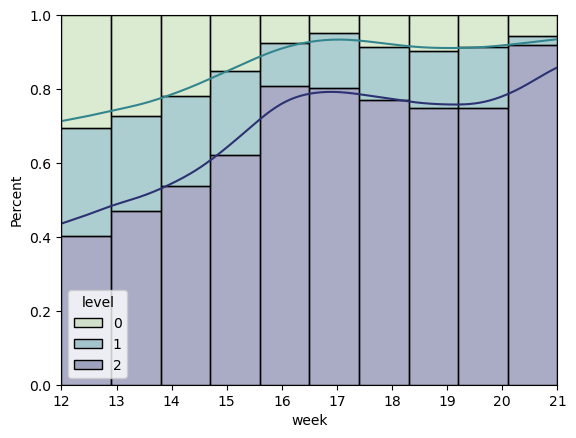
\includegraphics[width=0.45\linewidth]{Assets/not_skip_count.png}
}
% \caption{Random Forest}
% \label{fig_ShaplyRF}
% \end{subfigure}
% \hfill
% \begin{subfigure}[t]{0.24\textwidth}
\subfloat[Nghỉ học \label{feat_imb3}]{
    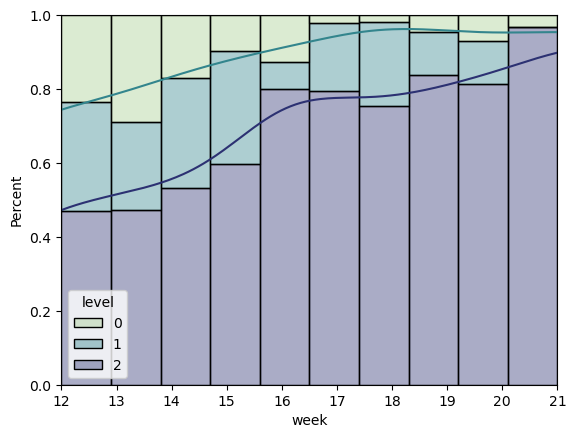
\includegraphics[width=0.45\linewidth]{Assets/skip_count.png}
}
% \caption{XGBoost model}
% \label{fig_ShaplyXG}
% \end{subfigure}
\caption{Biểu đồ tỉ số số lượng sinh viên theo trang thái tâm lý trong các tuần học đối với nhóm sinh viên có thực hiện (a) Không nghỉ học, (b) Nghỉ học trong ngày}
\label{feat_imp}
\end{figure}

Về các yếu tố học tập và thời gian, số lượng sinh viên bị căng thẳng cao có xu hướng chiếm phần lớn trong lượng sinh viên. Điều này là một vấn đề bình thường vì việc học thêm kiến thức hằng ngày tạo cho sinh viên áp lực khiến cho sinh viên có thể có những mệt mỏi dẫn đến căng thẳng. Ngoài ra, về số lượng sinh viên bị căng thẳng cao, hai nhóm sinh viên có nghỉ hocj và không nghỉ học có sự khác biệt lớn. Đối với nhóm nghỉ học, tỉ lệ sinh viên bị căng thẳng tăng đến tuần 16-17, tức tuần thi giữa kì, sau đó giữ nguyên. Còn đối với nhóm sinh viên còn lại, việc căng thẳng cao đạt đỉnh tại tuần 16-17. Điều này có thể do sinh viên đi học đầy đủ có điểm thi giữa kì tốt hơn và không chịu áp lực điểm thi cuối kì phải cao để qua môn còn với nhóm sinh viên nghỉ học phải chịu áp lực đó. Đặc biệt hơn, đối với sinh viên không nghỉ học, tỉ lệ sinh viên cảm thấy vui vẻ chiếm nhiều hơn so với nhóm sinh viên nghỉ học, thể hiện sinh viên đi học đầy đủ có thể phải chịu ít áp lực do học tập hơn nhóm còn lại. 

Một điều đáng quan tâm là yếu tố lý do cho sự nghỉ học. Về lý do nghỉ học cho các hoạt động bên ngoài, điều này là dấu hiệu của việc sinh viên bị căng thẳng tâm lý (hình \ref{feat_imp}). Để giải thích cho vấn đề này, việc sinh viên bị stress sẽ có xu hướng ra ngoài làm những việc thư giãn, điều này sẽ giúp cho sinh viên cảm thấy tốt hơn, dẫn đến những ngày có dữ liệu sinh viên nghỉ học để đi ra ngoài được gán với trạng thái tâm lý stress của sinh viên. Đặc biệt hơn việc nghỉ học để ở nhà lại có ít tác động đến sức khoẻ tinh thần của sinh viên hơn so với nghỉ học để cho các hoạt động bên ngoài. Theo tư duy thông thường, nhà là nơi để nghỉ ngơi và có thể là nơi để giải toả các vấn đề nhưng với cuộc sống sinh viên, thời gian ở nhà có thể được gán cho hai việc, nghỉ ngơi, hoặc hoàn thành các hạn nộp bài. Hai yếu tố này diễn ra trong cùng một loại vị trí và có tác động trái ngược nhau, vì vậy việc nghỉ học để ở nhà được phân tích gây nên yếu tố ở nhà có thể ảnh hưởng tích cực lẫn tiêu cực đến sức khoẻ tinh thần của sinh viên

\begin{figure}[!ht]
    \centering
    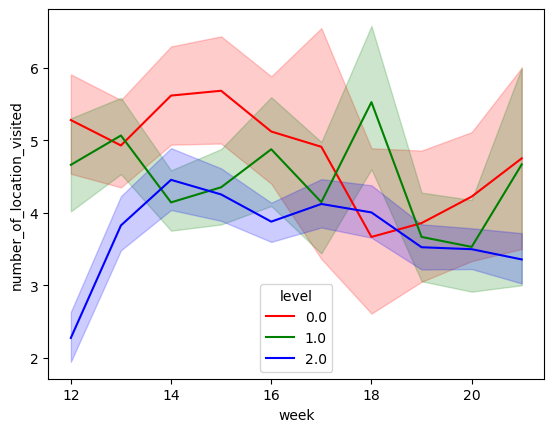
\includegraphics[width=0.75\linewidth]{num_of_loc_by_week.png}
    \caption{Biểu đồ biểu diễn số lượng địa điểm đến của sinh viên theo tuần chia theo mức độ căng thẳng}
    \label{num_of_loc_week}
\end{figure}

\begin{figure}[!ht]
    \centering
    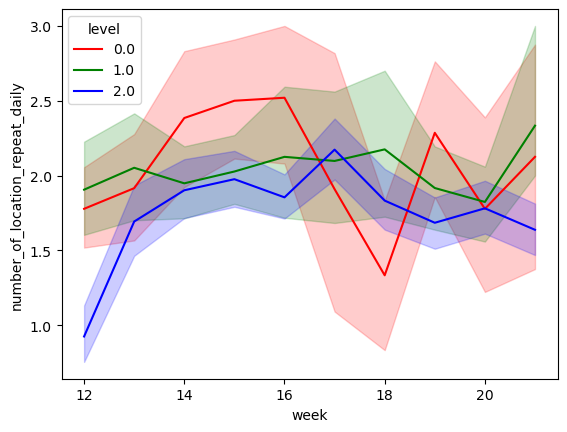
\includegraphics[width=0.75\linewidth]{num_of_location_daily_week.png}
    \caption{Biểu đồ biểu diễn số lượng địa điểm lặp lại trong 2 ngày liên tiếp của sinh viên theo tuần chia theo mức độ căng thẳng}
    \label{daily repeat}
\end{figure}

Một điều đáng chú ý khác là thói quen di chuyển của sinh viên. Phân tích đặc trưng chỉ ra rằng số lượng điểm đến ảnh hưởng tích cực với trạng thái của sinh viên. Lấy ví dụ một sinh viên có số lượng địa điểm đến trong một ngày thấp, điều này có thể chỉ ra người này chỉ làm việc trong một không gian nhất định, việc thiếu sự đổi mới sẽ có thể dẫn đến việc thiếu giao tiếp và dẫn đến stress. Ngược lại, nếu một người được ghi nhận ở nhiều địa điểm, điều này chứng tỏ người ấy đã di chuyển nhiều, và việc di chuyển sẽ giúp người đó có các tương tác xã hội, góp phần làm giảm căng thẳng tâm lý. 

Đặc biệt hơn, về yếu tố độ lặp lại của các trạng thái, sự lặp đi lặp lại theo hai ngày liên tục hoặc một ngày của hai tuần liên tiếp đạt giá trị vừa phải có thể là dấu hiệu người đó đang có trạng thái tâm lý thoải mái. Việc này có thể lý giải bằng hành vi của con người khi con người ta có nhiều sự lựa chọn, con người thường sẽ lựa chọn trải nghiệm, dẫn đến sự lặp lại giảm xuống. 

Đối chiểu với kết quả của nghiên cứu này, với nhóm sinh viên bị căng thẳng tâm lý nặng, nhóm sinh viên này có xu hướng di chuyển đến các địa điểm ít hơn so với các sinh viên khác (hình \ref{num_of_loc_week}). Ngoài ra nhóm này cũng ít khi thay đổi những điểm đến của mình (hình \ref{daily repeat}). Điều này vô hình làm cho sinh viên thiếu sự thay đổi trong các hoạt động trong ngày dẫn đến các vấn đề tinh thần như đã trình bày ở trên.


\begin{figure}[!ht]
    \centering
    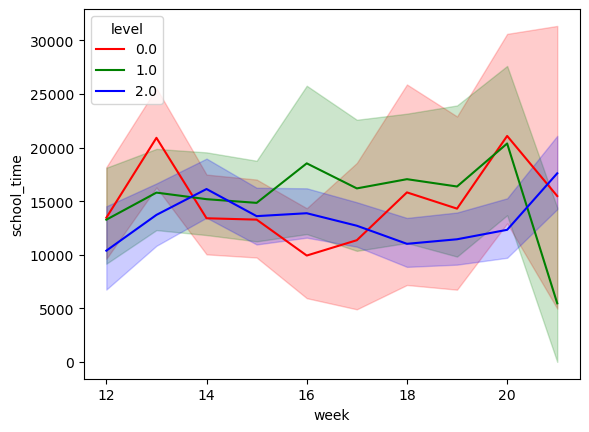
\includegraphics[width=0.75\linewidth]{Shooltime_week_line.png}
    \caption{Biểu đồ biểu diễn thời gian đi học của sinh viên theo tuần chia theo mức độ căng thẳng}
    \label{line_week_school}
\end{figure}
Ngoài ra, việc các thời gian giành cho các địa điểm cũng mang ý nghĩa nhất định đến việc căng thẳng tâm lý của sinh viên. Một ví dụ điển hình ở đây là phân tích về thời gian đi học. Thời gian đi học là một phần quan trọng với sinh viên khi đây là cơ hội để các sinh gặp được những người bạn, giáo sư của họ. Việc gặp gỡ và giao tiếp xã hội sẽ giúp cho các sinh viên giải toả được áp lực, từ đó sinh viên có thể cảm thấy tốt hơn. Cụ thể trong nghiên cứu này, hình \ref{line_week_school} đã thể hiện những sinh viên bị stress có xu hướng ở trường ít hơn sinh viên không bị căng thẳng tâm lý. Ngoài ra với nhhoms căng thẳng cao, nhóm này thường có thời gian đi học thấp nhất. Vì vậy có thể nhận thấy một mối tương quan giữa thời gian đi học và sức khoẻ tâm lý của sinh viên.

\begin{figure}[!ht]
    \centering
    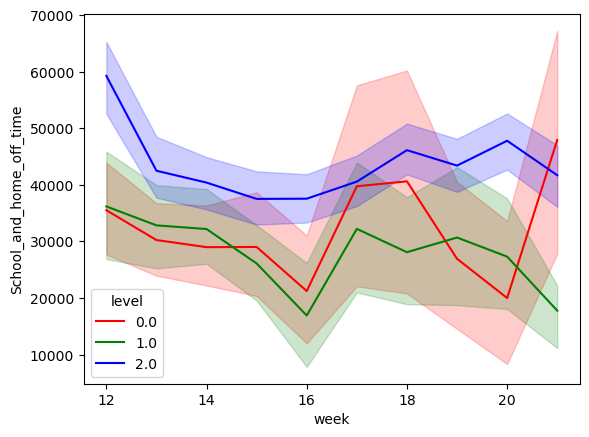
\includegraphics[width=0.75\linewidth]{line_week_home_a_school_off.png}
    \caption{Biểu đồ biểu diễn thời gian ở ngoài nhà và trường của sinh viên theo tuần chia theo mức độ căng thẳng}
    \label{line_week_homeaschooloff}
\end{figure}

Hơn thế, thời gian ngoài nhà và lớp học cũng đáng được quan tâm. Với thời gian này quá nhiều có thể gây nên những căng thẳng tâm lý. Như trong nghiên cứu này sinh viên gặp tình trạng căng thẳng cao (đường màu xanh dương hình \ref{line_week_homeaschooloff}) có thời gian ở ngoài nhà và trường nhiều nhất. Để lý giải vấn đề này, thời gian ở ngoài nhà và lớp học phản ánh khoảng thời gian sinh viên phải ở bên ngoài. Nếu sinh viên ở bên ngoài lâu, việc này sẽ làm mất cân bằng cuộc sống của sinh viên, và khi sinh viên này nhận ra còn việc làm ở nhà và ở trường sẽ gây ra trạng thái căng thẳng.


Vì vậy các yếu tố hành động, và các yếu tố hành vi khai thác từ hành động chứng minh được ý nghĩa trong việc đặc trưng cho cách mà sinh viên đối mặt với căng thẳng từ đó ta có thể lợi dụng điểm này để khai thác tạo nên các ứng dụng nhận diện sức khoẻ tinh thần dành cho sinh viên.



\newpage
\chapter{Tổng kết}
\section{Nhận xét}
Nghiên cứu này khám phá khả năng dự đoán của các mô hình học máy tận dụng các tính năng dựa trên GPS. Kết quả của tôi tiết lộ mối liên hệ đáng kể giữa mức độ căng thẳng của học sinh và các hành vi có thể nhận biết được thông qua dữ liệu điện thoại di động. Đặc biệt, các kỹ thuật học máy, đáng chú ý là mô hình Rừng ngẫu nhiên và XGB, cho thấy triển vọng trong việc phát hiện sớm và cảnh báo các vấn đề căng thẳng ở các cá nhân. Những phát hiện này cung cấp những hiểu biết quan trọng về dự đoán sức khỏe tâm thần, nhấn mạnh tầm quan trọng của các yếu tố như chỉ số tuần, thời gian giải trí, thời gian ở nhà, và thời gian học trong việc hiểu được căng thẳng tâm lý của học sinh.
\section{Hướng phát triển}
Về hướng phát triển, tôi đề xuất các nghiên cứu tiếp theo tập trung khai phá những yếu tố khác như thời lượng sử dụng điện thoại, quãng đường di chuyển, giấc ngủ, chủng tộc, sự thay đổi văn hoá (ở những đối tượng sinh viên trrao đổi văn hoá),... để có cái nhìn tổng quát hơn về vấn đề. Ngoài ra nghiên cứu này chỉ dừng lại ở các thuật toán học máy, các nghiên cứu tiếp theo có thể ứng dụng các giải thuật học sâu để có thể tìm ra được quy luật của trạng thái tâm lý.
\input{Contents/phuluc}


\bibliographystyle{ieeetr}

% \bibliographystyle{unsrtnat}
\bibliography{bib}
% \begin{thebibliography}{00}
% \bibitem{HSE} HSE on work related stress. 2016.Accessed: http://www.hse.gov.uk/statistics/causdis. 

% \bibitem{american stress} P. N. Alert, ”More Americans Rate Their Mental Health Worse Compared With a Year Ago, Poll Finds,” Psych News Alert, Dec. 22, 2022, https://alert.psychnews.org/2022/12/more-americans-rate-their-mental-health.html 

% \bibitem{stress_reduce_productivity} VanWormer, Jeffrey J; Fyfe-Johnson, Amber L. ND; Boucher, Jackie L, RD; Johnson, Pamela Jo PhD, MPH; Britt, Heather R, MPH; Thygeson, N. Marcus MD; Dusek, Jeffery A. Stress and Workplace Productivity Loss in the Heart of New Ulm Project. Journal of Occupational and Environmental Medicine 53(10):p 1106-1109, October 2011. DOI: https://doi.org/10.1097/JOM.0b013e318229ab18
 
% \bibitem{workday_lost}American Psychiatric Association, ”Americans Anticipate Higher Stress at the Start of 2023 and Grade Their Mental Health Worse,”
% \bibitem{PS}Pekka Siirtola. 2019. Continuous stress detection using the sensors of commercial smartwatch. In Adjunct Proceedings of the 2019 ACM International Joint Conference on Pervasive and Ubiquitous Computing and Proceedings of the 2019 ACM International Symposium on Wearable Computers (UbiComp/ISWC '19 Adjunct). Association for Computing Machinery, New York, NY, USA, 1198–1201. https://doi.org/10.1145/3341162.3344831
% \bibitem{d}
% M. Gjoreski, H. Gjoreski, M. Lutrek, and M. Gams, "Automatic Detection of Perceived Stress in Campus Students Using Smartphones", {\em in 2015 International Conference on Intelligent Environments (IE)}, pp. 132-135, 2015, doi: https://doi.org/10.1109/IE.2015.27.

% \bibitem{e}
% E. Vildjiounaite, J. Kallio, V. Kyllönen, et al., "Unobtrusive stress detection on the basis of smartphone usage data", {\em Perservative Ubiquitous Computing 22}, 671-688 (2018), doi: https://doi.org/10.1007/s00779-017-1108-z
% \bibitem{the Guardian}the Guardian (2014), Facebook reveals news feed experiment to control emotions
% \bibitem{stress_heartrate}M. Salai, I. Vassányi, and I. Kósa, ‘Stress detection using low cost heart rate sensors’, J. Healthc. Eng., vol. 2016, pp. 1–13, 2016.
% \bibitem{stress_def}Hobfoll, S. E. (1998). Stress, culture, and community: The psychology and philosophy of stress. Plenum Press. https://doi.org/10.1007/978-1-4899-0115-6
% \bibitem{Stress thermo} Yi Xiaoet al. (2024), Reading Between the Heat: Co-Teaching Body Thermal Signatures for Non-intrusive Stress Detection. Proc. ACM Interact. Mob. Wearable Ubiquitous Technol. 7, 4, Article 189 (December 2023), 30 pages. https://doi.org/10.1145/3631441
% \bibitem{student life}
% R. Wang et al., "StudentLife: Assessing mental health, academic performance and behavioral trends of college students using smartphones," {\em in Proceedings of the 2014 ACM International Joint Conference on Pervasive and Ubiquitous Computing}, pp. 3-14, 2014.
% \bibitem{student life2}Xuhai Xu et al. (2023), GLOBEM: Cross-Dataset Generalization of Longitudinal Human Behavior Modeling. Proc. ACM Interact. Mob. Wearable Ubiquitous Technol. 6, 4, Article 190 (December 2022), 34 pages. https://doi.org/10.1145/3569485
% \bibitem{student life4} Weichen Wang, Subigya Nepal, Jeremy F. Huckins, Lessley Hernandez, Vlado Vojdanovski, Dante Mack, Jane Plomp, Arvind Pillai, Mikio Obuchi, Alex daSilva, Eilis Murphy, Elin Hedlund, Courtney Rogers, Meghan Meyer, and Andrew Campbell. 2022. First-Gen Lens: Assessing Mental Health of First-Generation Students across Their First Year at College Using Mobile Sensing. Proc. ACM Interact. Mob. Wearable Ubiquitous Technol. 6, 2, Article 95 (July 2022), 32 pages. https://doi.org/10.1145/3543194


% \bibitem{Muller}
% P. Müller et al., "Analyzing GPS data for psychological research: A Tutorial", {\em Advances in Methods and Practices in Psychological Science}, vol. 5, no. 2, pp. 25152459221082680, 2022.

% \bibitem{Shikha}Shikha, D. D. Sethia and S. Indu, "Optimization of Wearable Biosensor Data for Stress Classification Using Machine Learning and Explainable AI," in IEEE Access, doi: 10.1109/ACCESS.2024.3463742.

% \bibitem{student life3}Subigya Nepal et al. (2024), Capturing the College Experience: A Four-Year Mobile Sensing Study of Mental Health, Resilience and Behavior of College Students during the Pandemic. Proc. ACM Interact. Mob. Wearable Ubiquitous Technol. 8, 1, Article 38 (March 2024), 37 pages. https://doi.org/10.1145/3643501
% \bibitem{school_time_and_stress}Verma, S., Sharma, D. and Larson, R. W. (2002) ‘School stress in India: Effects on time and daily emotions’, International Journal of Behavioral Development, 26(6), pp. 500–508. doi: 10.1080/01650250143000454.

% \bibitem{rf} G. Biau and E. Scornet, “A Random Forest Guided Tour - Test,” SpringerLink, https://link.springer.com/article/10.1007/s11749-016-0481-7 (accessed Feb. 23, 2024).

% \bibitem{xgb} XGBoost Documentation. (2022). Accessed: Feb 3, 2024.[Online]. Available: https://xgboost.readthedocs.io/en/stable/\#xgboost-documentation

% \bibitem{SVM} Cortes, C. \& Vapnik, V. Support-vector networks. {\em Machine Learning}. \textbf{20}, 273-297 (1995)
% \bibitem{SMOTE} G. A. Pradipta, R. Wardoyo, A. Musdholifah, I. N. H. Sanjaya, and M. Ismail, "SMOTE for Handling Imbalanced Data Problem: A Review," {\em 2021 Sixth International Conference on Informatics and Computing (ICIC)}, pp. 1-8, doi: 10.1109/ICIC54025.2021.9632912.

% \bibitem{T-links}Elhassan, T., M, A., F, A. \& Shoukri, M. Classification of Imbalance Data using Tomek Link (T-Link) Combined with Random Under-sampling (RUS) as a Data Reduction Method. {\em Global Journal Of Technology And Optimization}. \textbf{1} (2016,1)

% \bibitem{ENN}Tang, B. \& He, H. ENN: Extended Nearest Neighbor Method for Pattern Recognition [Research Frontier]. {\em IEEE Computational Intelligence Magazine}. \textbf{10}, 52-60 (2015)

% \bibitem{tree explainer} S. M. Lundberg et al., "From local explanations to global understanding with explainable AI for trees",{\em Nature Machine Intelligence}, vol. 2, no. 1, pp. 56–67, Jan. 2020, doi: https://doi.org/10.1038/s42256-019-0138-9.

% \bibitem{shap value} S. Fadel, "Explainable Machine Learning, Game Theory, and Shapley Values: A Technical Review," arXiv preprint arXiv:2202.13535, 2022.

% \bibitem{LIME}M. T. Ribeiro, S. Singh, and C. Guestrin, “Why Should I Trust You?”: Explaining the Predictions of Any Classifier. 2016. [Online]. Available: https://arxiv.org/abs/1602.04938

% \bibitem{Herbert}Herbert, T.B. and Cohen, S. (1993) Stress and Immunity in Humans: A Meta-Analytic Review. Psychosomatic Medicine, 55, 364-379.
% http://dx.doi.org/10.1097/00006842-199307000-00004

% \bibitem{Lazarus}Lazarus, R. S. (1993). From psychological stress to the emotions: A history of changing outlooks. Annual Review of Psychology, 44, 1–21. https://doi.org/10.1146/annurev.ps.44.020193.000245
% \bibitem{Youngjun}Youngjun Cho and Nadia Bianchi-Berthouze. 2019. Physiological and affective computing through thermal imaging: A survey. arXiv
% preprint arXiv:1908.10307 (2019).
% \bibitem{Alan}Alan T Krzywicki, Gary G Berntson, and Barbara L O’Kane. 2014. A non-contact technique for measuring eccrine sweat gland activity using passive thermal imaging. International journal of psychophysiology 94, 1 (2014), 25–34.
% \bibitem{eustress distress}J. Bienertova-Vasku, P. Lenart, M. Scheringer, Eustress and Distress: Neither Good Nor Bad, but Rather the Same?. BioEssays 2020, 42, 1900238. https://doi.org/10.1002/bies.201900238
% \bibitem{eustress distress2}Le Fevre, M., Matheny, J. and Kolt, G.S. (2003), "Eustress, distress, and interpretation in occupational stress", Journal of Managerial Psychology, Vol. 18 No. 7, pp. 726-744. https://doi.org/10.1108/02683940310502412

% \bibitem{eustress distress3}C. Sandi and M. T. Pinelo-Nava, "Stress and memory: behavioral effects and neurobiological mechanisms," Neural Plast., vol. 2007, no. article number 78970, pp. 1-9, 2007. [Online]. Available: https://doi.org/10.1155/2007/78970
% \bibitem{eustress distress4} N. Schneiderman, G. Ironson, and S. D. Siegel, "Stress and Health: Psychological, Behavioral, and Biological Determinants," Ann. Rev. Clin. Psychol., vol. 1, pp. 607-628, 2005. 
% \bibitem{cortisol}Lee DY, Kim E, Choi MH. Technical and clinical aspects of cortisol as a biochemical marker of chronic stress. BMB Rep. 2015 Apr;48(4):209-16. doi: 10.5483/bmbrep.2015.48.4.275. PMID: 25560699; PMCID: PMC4436856.
% \bibitem{datetime_lib} Python Documentation, datetime — Basic date and time types, [Online]. Available: https://docs.python.org/3/library/datetime.html
% \end{thebibliography}


\newpage
\appendix
\chapter{Các công bố khoa học cho đồ án này}
% the \\ insures the section title is centered below the phrase: AppendixA
Một phần đồ án này được trình bày tại ABC 2023 và ISAS 2024.

\begin{figure}[!ht]
    \centering
    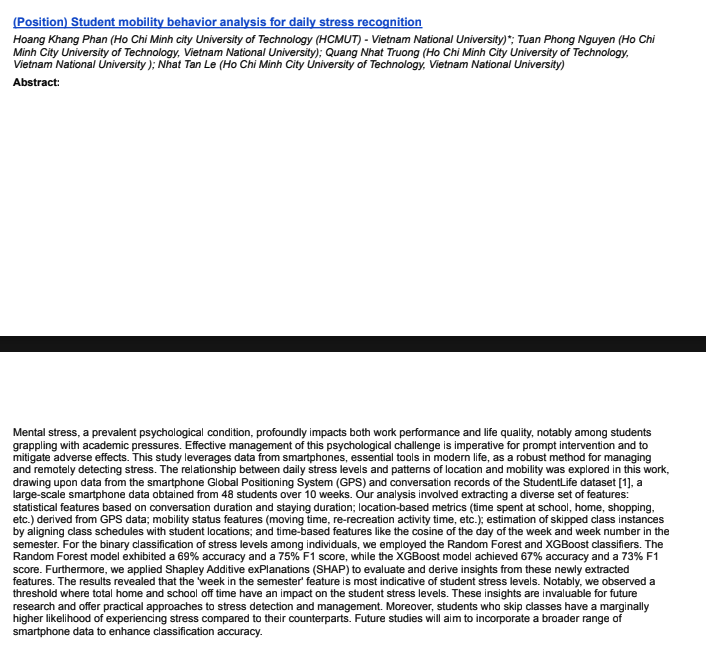
\includegraphics[width=\linewidth]{acb2024.png}
\end{figure}



\end{document}


